\documentclass[twoside,a4paper,11pt]{article}
\usepackage{wrapfig}
\usepackage{graphicx}
\usepackage{graphics}
\usepackage{amsmath}
\usepackage{amsfonts}
\usepackage[T1]{fontenc}
\usepackage{amssymb}
\usepackage[font=footnotesize, singlelinecheck=false, labelfont=bf]{caption}
\usepackage{array}
\usepackage{multirow}
\usepackage{setspace}
\usepackage{hyperref}
\usepackage{verbatim}
\usepackage{epstopdf}
\usepackage{textcomp}
\usepackage{nicefrac}
\usepackage{xspace}
\usepackage{lineno}
\usepackage[footnotesize, bf, hang, raggedright]{subfigure}
\usepackage{charter}
\usepackage[expert]{mathdesign}
\usepackage[bottom]{footmisc}
\usepackage[english]{babel}
\usepackage{tikz}
\usetikzlibrary{arrows}

\onehalfspacing
\usepackage[left=2.9cm,right=2.9cm,top=3cm,bottom=4.5cm]{geometry}

\newcommand{\subfigureautorefname}{\figurename}
\newcommand\geant{\textsc{Geant\,4}\xspace}
\newcommand\mokka{\textsc{Mokka}\xspace}
\newcommand\ddhep{\textsc{DD4hep}\xspace}

\usepackage{xcolor}
\usepackage[printwatermark]{xwatermark}
\newwatermark[allpages,color=gray!30,angle=45,scale=3,xpos=-10,ypos=0]{Draft}

\usepackage{titlesec} 
\titleformat{\section}[hang]{
\usefont{T1}{qhv}{b}{n}\selectfont} % "qhv" - TeX Gyre Heros, "b" - bold
{} 
{0em}
{\hspace{-0.4pt}\Large \thesection\hspace{0.6em}}

\usepackage[subfigure]{tocloft} % subfigure option only if using subfigure package
\renewcommand{\cfttoctitlefont} % ToC title
             {\usefont{T1}{qhv}{b}{n}\selectfont\huge}
\renewcommand{\cftsecfont} % section titles
             {\usefont{T1}{bch}{b}{n}\selectfont}
\renewcommand{\cftsubsecfont} % subsection titles
             {\usefont{T1}{bch}{m}{n}\selectfont} 
\renewcommand{\cftsecpagefont} % section page numbers
             {\cftsecfont} 
\renewcommand{\cftsubsecpagefont} % subsection page numbers
             {\cftsubsecfont}

\linenumbers
\setcounter{tocdepth}{2}

\begin{document}
\selectlanguage{english}
\begin{titlepage}
\begin{flushright}
CALICE Analysis Note CAN-057\\
v1.0\\
October 7, 2016 \\
\end{flushright}

\begin{center}
\vspace*{\fill}
\begin{LARGE} \textbf{Timing Resolution in Testbeam of the CALICE Analog Hadronic Calorimeter} \end{LARGE} \\ [10ex]
\begin{Large} The CALICE Collaboration \footnote{Corresponding authors: \\ Eldwan Brianne; eldwan.brianne@desy.de; Katja Krueger; katja.krueger@desy.de}\\ [10ex]
\end{Large}

\begin{large}
\textbf{Abstract} \\
\end{large}
\end{center}
This note presents results obtained with the CALICE engineering prototype consisting of the \emph{Analog Hadronic Calorimeter} at the CERN testbeam campaign in 2015. The analysis includes timing distributions for muon, electron and pion beams. The results are compared to several \geant version 10.1 physics lists.\\
\\

\textit{
This note contains preliminary CALICE results, and is for the use of members of the CALICE Collaboration and others to whom permission has been given.}

\end{titlepage}

\clearpage
\tableofcontents
\newpage
\section{Introduction}

The International Large Detector (ILD) considers a highly granular hadronic calorimeter using iron absorbers to achieve a compact detector with the best jet energy resolution around 3-4\% at 250 GeV satisfying the space constrain imposed by the solenoid magnet. Timing measurements in a calorimeter can be used to reject pile-up events like at the LHC or CLIC due to the bunch-to-bunch spacing of 25 and 0.5 ns respectively. Also the high level of $\gamma\gamma \rightarrow$ hadrons could be rejected by using timing information of the calorimeter in order to limit the impact of the background on physics measurements.\\
In the hadronic calorimeter, the timing precision is highly influenced by the time structure of the shower itself. A hadronic shower possesses several timing components related to different processes happening in the shower. A fast component related to instantaneous highly energetic deposits from high-energy hadrons and electromagnetic sub-showers. A slow component due to neutron scattering, nuclear-recoil and photons from nuclear processes, this component can last up to several milliseconds. Apart from physics processes, the time structure of the shower is influenced by the active medium used as well as the electronics. Time constants in the active medium such as scintillation decay time can affect the measurement.\\
The performance of the ILD relies on simulation studies based on \geant, it is important to study how well the simulation performs to reproduce the time structure of hadronic showers observed in data. The CALICE Analog Hadronic Calorimeter (AHCAL) technological prototype has been installed in the SPS CERN facilities in July and August 2015 in order to provide measurements using plastic scintillators.

\section{The CERN 2015 Testbeam Setup}

The datasets used in this note were collected during the testbeam campaign at CERN Super Proton Synchrotron (SPS) in July 2015. The SPS beamline provides secondary beams of hadrons, electrons and muons in a wide particle momenta range from 10 to 360 GeV/c. More details on the beamline are available in \cite{SPSBeamLine}.

\subsection{The CALICE AHCAL technological prototype}

In the July 2015 testbeam period, the CALICE AHCAL is a sandwich-based calorimeter consisted of 38 iron absorber plates, 19 mm thick corresponding to a depth of approximately 40 $X_0$ ($\sim$ 4.5 nuclear interaction length $\lambda_{n}$). The active layer is consisted of a iron cassette, 1 mm thick, a HCAL Base Unit (HBU) of an area of $36\times36$ cm$^2$, hosting the integrated readout electronics and a $30\times30\times3$ mm$^3$ plastic scintillator tile wrapped in a reflective foil. Each plastic tiles are read out individually by a SiPM, corresponding to 3744 channels total.
The prototype used was not fully equipped only 14 layers were inserted as illustrated in figure \ref{fig:detector_layout}. 
%\begin{tikzpicture}[scale=1]
%
%\draw [line width=0.5mm,  black] (3.4,-0.2) -- (3.4, 0.2);
%\draw [line width=0.5mm,  black] (3.6,-0.2) -- (3.6, 0.2);
%\draw [line width=0.5mm,  black] (3.8,-1) -- (3.8, 1);
%\fill[gray!40!white] (4,-0.5) rectangle(4.9,0.5);
%\fill[gray!40!white] (5,-1) rectangle(8,1);
%\draw [line width=0.5mm,  black] (8.2,-1) -- (8.2, 1);
%\draw[thick,->] (0,0) -- (10,0) node[anchor=north east] {z};
%
%\end{tikzpicture}
\begin{figure}[htbp]
	\subfigure[Picture of the AHCAL steel stack during the CERN testbeam.\label{fig:stack_steel}] {\includegraphics[width=0.35\textwidth]{fig/steel_stack_ps.png}}\hfill
	\subfigure[Detector layout of the CALICE AHCAL during the 2015 July Testbeam at the SPS.\label{fig:detector_layout}] {\includegraphics[width=0.60\textwidth]{fig/Detector_layout.png}}
	\caption[]{\textbf{a}: Picture of the CALICE AHCAL during the Testbeam in July 2015 at CERN. The trigger scintillators can be seen in front of the stack in the photo. \textbf{b}: Layout used during the July 2015 SPS Testbeam campaign.}
	\label{fig:full_detector_layout}
\end{figure}
\subsection{Testbeam Setup}

The two first layers were consisted of ECAL Base Unit (EBU) with 144 scintillator strips of $45\times5\times2$ mm$^3$ read out by SiPMs for a total area of $18\times18$ cm$^2$. The next 8 layers are consisted of a single HBU are used as a shower start finder in order to locate the first hard hadronic interaction. And the last 4 layers are consisted of $2\times2$ HBUs in order to study timing of hadronic showers. The prototype was equipped by various electronics and tile designs that are sum up in the following table \ref{table:sipm_list}:
\begin{table}[htbp]
\centering
    \begin{tabular}{@{} cccccc @{}}
    \hline
    Layer \# & Model & Area (mm$^2$) & Pitch ($\mu$m) & WLS Fiber & Read out \\ \hline
    1 & S12571\_010P & $1\times1$ & 10 & no & Bottom \\ 
    2 & S10362-11-025O & $1\times1$ & 25 & no & Side \\
    3 & S12571-025P & $1\times1$ & 25 & no & SMD \\ 
    4-5 & N/A & $2.25\times2.25$ & 18 & no & Side \\
    6-10 & CPTA & $1.28\times1.28$ & 40 & yes & Side \\ 
    11-12 & PM1125NS-SB0 & $1.2\times1.2$ & 25 & no & Side \\
    13-14 & MicroFB-10020-SMT & $1\times1$ & 20 & no & Side \\
    \hline
    \end{tabular}
     \caption{List of the different SiPMs used in the CALICE AHCAL in July 2015.}
     \label{table:sipm_list}
\end{table}
\subsection{The SPIROC2B chip}

The SiPMs are read out by a SPIROC2B chip which features 36 channels measuring ADC amplitudes (energy) and TDC amplitudes (time) and can store up to 16 events. The collected charge from the SiPM is stored in a capacitor (memory-cell) waiting to be digitised with a 12 bit range. The chip can be configured in 2 different modes. External trigger mode is used for gain calibration via an integrated LED Calibration System and monitoring of the SiPM. Auto-trigger mode is used to collect physics data, a threshold of 0.2-0.5 MIP is set for each chips in the setup.
The time is measured via a fast shaper when the signal passes the threshold and is digitised by a voltage ramp. Each chip possesses two voltage ramps that are multiplexed when a new Bunch Crossing (BXID) occurs. The length of a BXID is defined by the slow clock of the chip. In testbeam, the clock used is of 250 kHz which would correspond to a BXID length of 4 $\mu$s but due to the ramp multiplexer a dead time of around 2\% has to be taken into account. Thus the ramp length is of 3.92 $\mu$s.\\
\begin{figure}[htbp]
\begin{center}
\includegraphics[width=0.6\textwidth]{fig/Spiroc_layout.png}
\caption{Schematic of the signal path of the SPIROC2B for a single channel.}
\label{fig:SPIROC2B}
\end{center}
\end{figure}
\subsection{Trigger Signals}
\label{subsec:trigger}

For Muon beam, two scintillator plates of $80\times80$ cm$^2$ were placed in front and back of the calorimeter. For electron and pion beams, two small scintillator plates of $30\times30$ cm$^2$ were positioned in front of the calorimeter (see figure \ref{fig:stack_steel}). The trigger scintillators were connected to a NIM-logic (discriminator and gate) in order to provide a validation of the data to the chip. 
In order to provide the time reference of the triggers, a SiPM-like pulse of around 4 $\mu$s period and with a fast rising edge around 1 ns was generated from the NIM-logic. This signal was injected directly via AC coupling to some channels in the setup as shown in the table \ref{table:trigger_signal_list}. 
\begin{table}[htbp]
\centering
  \begin{tabular}{@{} ccccc @{}}
    \hline
    Layer \# & Chip Number & Channel & Comments & Appellation \\ 
    \hline
    11 & 169 & 29 & noisy & T$_{11}$ \\ 
    11 & 177 & 23 & broken & - \\
    12 & 185 & 29 & - & T$_{12}$ \\ 
    13 & 201 & 29 & -  & T$_{13}$ \\
    13 & 211 & 6 & broken & - \\ 
    14 & 217 & 23 & - & T$_{14}$ \\
    \hline
  \end{tabular}
  \caption{List of channels with the injected trigger signal to be used as time reference.}
  \label{table:trigger_signal_list}
\end{table}
In the following analysis, only the reference signals T$_{12}$,  T$_{13}$ and T$_{14}$ were used.

\section{Simulation}

\subsection{AHCAL Simulation Model \& Digitisation}

The simulation of the testbeam prototype is based on the \mokka framework v08-05-01 and the new \ddhep framework v00-16, which provides a full \geant v10-1 based simulations of the detector implementations with detailed geometry and material descriptions. The right handed coordinate is used such as the Z-axis points out in the beam direction and that the Y-axis is directed upwards. No beamline instrumentation is simulated. This analysis uses the sub-detector \mokka models \textit{TBecal4d} for the ScECAL and \textit{TBhcal4d} for the AHCAL. The distance between the sub-detectors is set to 0 mm. In \ddhep, the compact and material description files are available in the \textit{calice\_dd\_testbeams} package of the CALICE development software. A check was performed between \mokka and \ddhep models with electrons and pions to ensure that the material description in both models are the same. A full validation of the AHCAL simulation model is still on-going.\\
The beam gun is placed 6 m in front of the calorimeter face for the simulations in this analysis. It is configured to generate single beam particle with no momentum spread and the beam profile for electrons and pions is extracted from data and applied to simulation for each individual runs. For muon runs, a flat beam covering the full AHCAL is simulated. As this is not expected to have an influence on the MIP and time response of the detector.
All electrons simulations are simulated with \geant 10.1 using the QGSP\_BERT physics list.\\
Pion showers are simulated using QGSP\_BERT, QGSP\_BERT\_HP and FTFP\_BERT\_HP physics lists as theses physics lists are well validated for the simulation of high energy showers. The package \textit{high precision} (\_HP) is used in order to understand the differences induced in timing with a precise treatment of the neutrons.\\
For each runs, 100 000 simulated $\mu^-$, $e^-$ and $\pi^-$ single particle events are generated.\\

The digitisation of simulated hits is very similar to the one used in the ScECAL and AHCAL physics prototypes \cite{CAN-002, CAN-010, JINST-6}. Using, if available, individual calibration factors obtained from data to extract the light yield which is needed to model the statistical fluctuations of photons hitting a SiPM. Saturation effects are also included using the number of pixels available on each SiPM type. This effect is still under study, should have negligible effects on timing thus is not used in the following analysis. Most of the tiles used are wrapped with a reflective foil in order that crosstalk effect between channels can be neglected. The timing is modelled in a same way as in the SPIROC, the energy from sub-hits in a cell is integrated over a sliding time window of 15 ns, if the energy sum passes the threshold the time of the simulated sub-hit passing the threshold is registered as the time of the hit. In order to simulate detector resolution effects, the time of a hit is smeared with a gaussian for each individual layer. Noise is an issue with the engineering AHCAL prototype as only hits above the trigger threshold are registered during a beam spill, noise hits are rejected in testbeam if no validation from the scintillator triggers is given to the DAQ \cite{DAQ}. A study of the effect of noise on timing is described in appendix \ref{appendix:noise_timing}.\\
After digitisation, simulated hits have the same format as raw data hits and are then reconstructed using the same software chain used for data. To suppress noise hits, only hits above 0.5 MIP as considered in this analysis in both simulation and data.

\section{Timing Calibration}
To perform the timing calibration of the AHCAL. The complete muon dataset is used. The electron dataset is used in a next step to validate the calibration procedure as described in subsection \ref{subsec:validation}. The following table \ref{table:mu_elec_runs} sums up the runs and datasets used. The number of raw events are counted if containing all the three trigger signals.
\begin{table}[htbp]
\centering
  \begin{tabular}{@{} cccccc @{}}
    \hline
    Runs & Energy & Particle Type & Events (raw) & Events (sel.) & $\frac{\text{N$_{sel.}$}}{\text{N$_{raw}$}}$ \\ 
    \hline
     24016 - 24663 & 50-150 GeV & $\mu^-$ & 990161 & 845797 & 85.4\% \\ 
     24487 & 20 GeV & $e^-$ & 29729 & 25589 & 86\% \\
    \hline
  \end{tabular}
  \caption{Table with the statistic before and after selection used for timing calibration.}
  \label{table:mu_elec_runs}
\end{table}
\subsection{Muon Selection}

The $\mu$ runs were taken first at 50 GeV then another scan at the end of the campaign was performed at 150 GeV. As the H2 beam line did not have any beam shutter, the muon beam was made by scrapping the halo of a secondary pion beam using collimators. Due to wrong configuration of the beamline, the muon runs were contaminated by pions. A first estimation provided that around 30\% of the events were contaminated. The main goal of the muon selection was to efficiently select muons and reject pion showers. For this, a simple track finder has been developed. In order to select muons or punch-through pions, a straight track of at least 7 hits is required in the whole AHCAL without a hard interaction. In addition to reject late pion showers, not more than 2 hits are required per layer.

\subsection{Electron Selection}
\label{subsec:elec_sel}

To perform comparisons on electron, a sample of electron events is selected from the data runs. A simple selection is performed in order to have mostly contained showers in the AHCAL. The selection requires at least 50 hits in the AHCAL, a fiducial cut of $80\times80\times360$ mm$^3$ on the center of gravity of the shower in x, y and z is made and less than 0.1\% of the energy sum should be contained in the last two layers.

\subsection{Slope calibration}
\label{subsec:slope_calib}

The data analysis is performed in several steps. The first step is the calibration of the time provided by the SPIROC2B chip. To reconstruct the time of the first hit in a channel, the TDC value measured needs to be converted into nanoseconds. The value is converted using the following equation:
\begin{equation} \label{eq:slope}
 \text{slope}_{chip, BXID} \: \text{[ns/TDC]} = \frac{3920 \: \text{ns}}{\text{Max}_{chip, BXID} - \text{Pedestal}_{chip, BXID}}
\end{equation}
\begin{equation} \label{eq:time_chn}
\text{T}_{chn} \: \text{[ns]} = \text{slope}_{chip, BXID} \times (\text{TDC}_{chn, mem} - \text{Pedestal}_{chn, mem} )
\end{equation}
The parameters Max$_{chip, BXID}$ and Pedestal$_{chip, BXID}$ in eq.\ref{eq:slope} are extracted from the TDC spectrum from a specific chip and BXID using only the first memory cell as illustrated in figure \ref{fig:TDC_Spectrum}. At the same time, the parameter Pedestal$_{chn, mem}$ in eq.\ref{eq:time_chn} is extracted from the spectrum for each channel and each memory cell of a chip and BXID. This is accounting for a total of 208 slopes and 119808 pedestals to be extracted for the testbeam setup.
\begin{figure}[htbp]
	\subfigure[TDC Spectrum of a typical chip.\label{fig:TDC_Spectrum}] {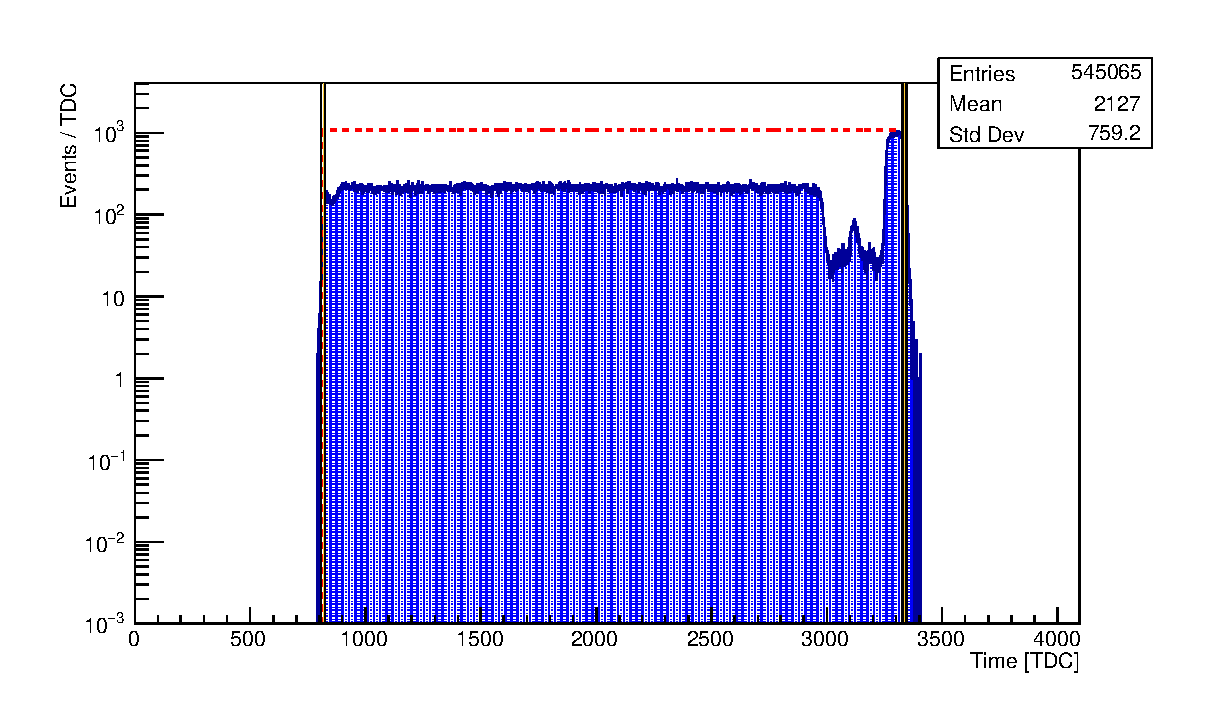
\includegraphics[width=0.5\textwidth]{fig/ExampleTDCSpectra.eps}}\hfill
	\subfigure[Distribution of the extracted TDC slopes.\label{fig:slope_time}] {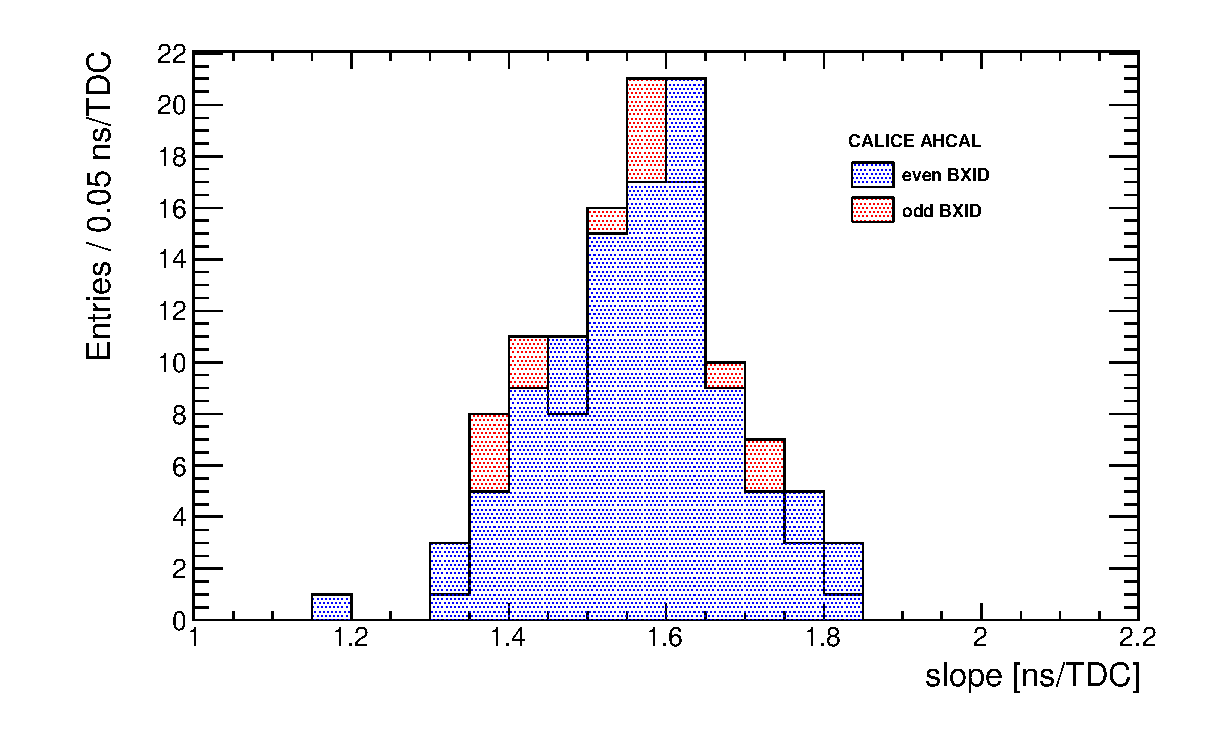
\includegraphics[width=0.5\textwidth]{fig/SlopeDistribution.eps}}
	\caption[]{\textbf{a}: The red rectangle are the fitted Max and Pedestal parameters for this chip. The yellow bands represents estimation of the error made on the extraction of the parameters by a variation of 1 RMS of the threshold $\mu$. The parameters extracted are slope = 1.56 $\pm$ 0.01, Pedestal = 816 $\pm$ 9 and Maximum = 3336 $\pm$ 8. \textbf{b}: Distribution of the fitted slopes $\mu_{odd}$ = 1.564, RMS$_{odd}$ = 0.121, $\mu_{even}$ = 1.556, RMS$_{even}$ = 0.113.}
\end{figure}
The technique of extraction is based on a edge detection method. For each chip and BXID, an histogram is filled with the content of each bin then the mean is defined as a threshold $\mu$. The parameter Pedestal$_{chip, BXID}$ is extracted as the first bin above 30\% of $\mu$. For the parameter Max$_{chip, BXID}$, it is extracted by taking 50\% of the maximum bin of the original histogram. An estimation of the errors made on the pedestal and maximum is done by variating the value of $\mu$ and the value of the maximum bin by 1 RMS and 33\% respectively.
The extracted values for the slopes are in the expected range of 1.6 ns per TDC bin due to the limited dynamic range provided by the chip (around 2500 bins for 4 $\mu$s). More details about the estimations of the calibration errors is described in the appendix \ref{appendix:calib_error}.

\subsection{Reconstruction of the hit time}

To reconstruct the time of the first hit in a channel, the measured time of a hit needs to be compared to the time of the reference trigger. The triggers signals described in subsection \ref{subsec:trigger} are calibrated using the same method as explained above. After time calibration of the hit, events are selected by requiring that T$_{12}$, T$_{13}$ and T$_{14}$ are present in the event in a certain amplitude range to reject noise hits from theses channels. Moreover, as theses channels receive exactly the same signal from the NIM-logic at the same time, a correction is applied to force them to match in time. The correction is performed by correcting the time of T$_{12}$ and T$_{13}$ compared to the time of T$_{14}$. The figure \ref{fig:T0_Correction} shows that the correction reduces slightly the spread of the trigger channels w.r.t to each other.
\begin{figure}[htbp]
\begin{center}
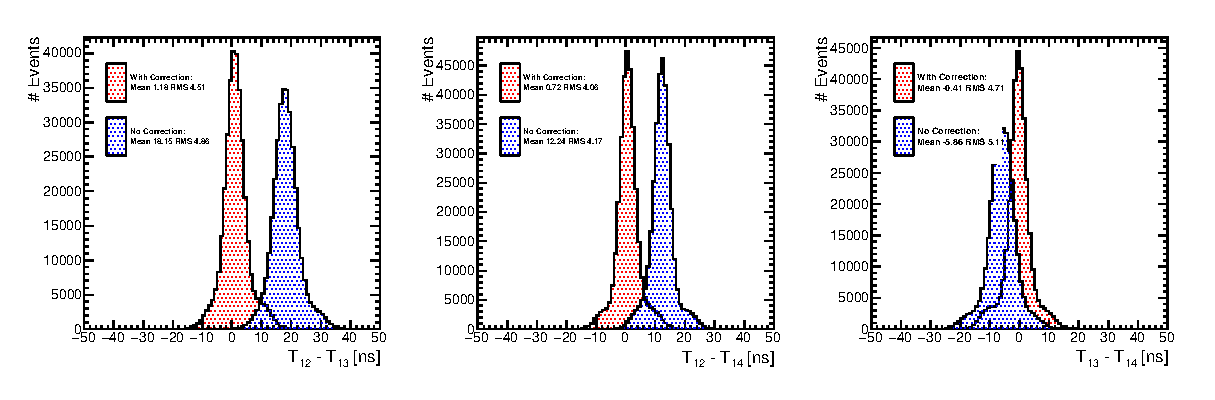
\includegraphics[width=1.0\textwidth]{fig/T0s_Resolution_2.eps}
\caption{Time difference between the trigger channels before and after correction.}
\label{fig:T0_Correction}
\end{center}
\end{figure}
In a next step, to reject wrong or late triggers and reduce the uncertainty made on the time of the trigger, the time reference $T_{ref}$ is calculated using the mean of T$_{12}$, T$_{13}$ and T$_{14}$ and its associated error $\sigma_{ref}$ as shown in eq. \ref{eq:tref} \& \ref{eq:tref_err}. A cut of 4 ns is performed on $\sigma_{ref}$ to reject events with a too large error on the time of the trigger.
\begin{equation} \label{eq:tref}
\text{T}_{ref} = \frac{\text{T}_{12} + \text{T}_{13} + \text{T}_{14}}{3}
\end{equation}
\begin{equation} \label{eq:tref_err}
\sigma_{ref} = \frac{ (\text{T}_{12} - \text{T}_{ref})^2 + (\text{T}_{13} - \text{T}_{ref})^2  + (\text{T}_{14} - \text{T}_{ref})^2 }{6}
\end{equation}
Since the absolute time between the passage of a muon and the trigger of a channel is not known, the timing relative to the trigger is determined from data. As muons are quasi-instantaneous particles thus the time of the first hit distribution for each channel and memory cells has to be shifted to \textit{t=0}. This shifting procedure takes into account the delay time of the trigger due to cabling and the NIM-logic as well as mis-calibrations in memory cell pedestals. Only channels containing more than 100 events are considered. As different trigger configurations were used for different data samples, each sample (muons, electrons and pions) has to be shifted separately. A distribution of the extracted offset can be seen in figure \ref{fig:offset_trigger_distribution}. The error made on the shift is estimated to be in the order of 1-2 ns.\\
After the selection, the time of the first hit (T$_{fH}$) can be obtained by plotting the distribution of T$_{chn}$ - T$_{ref}$ for each layer as shown on figure \ref{fig:layer3_time_shifted}.
\begin{figure}[htbp]
	\subfigure[Distribution of the offset used to correct for the trigger delay.\label{fig:offset_trigger_distribution}] {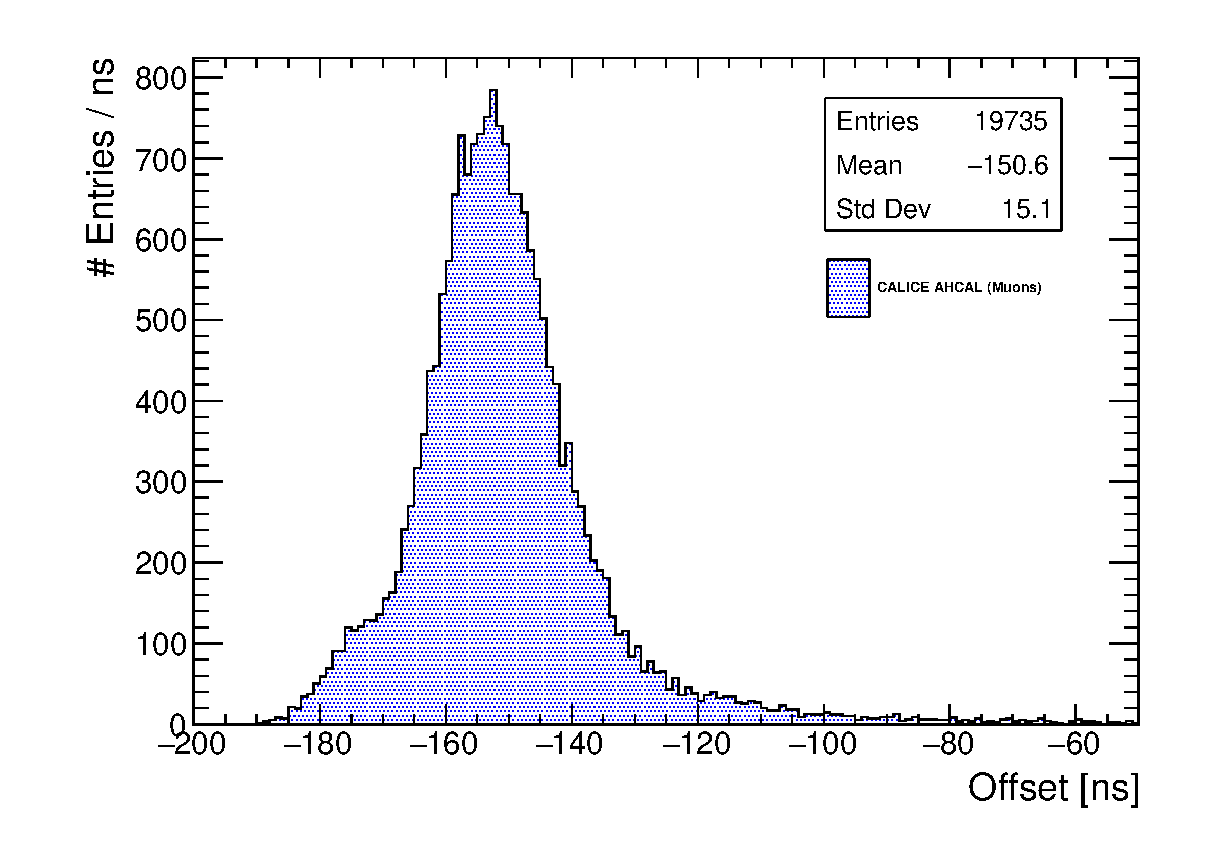
\includegraphics[width=0.5\textwidth]{fig/FittedOffsets.eps}}\hfill
	\subfigure[Time of the first hit distribution for Layer 3 after the shift to zero.\label{fig:layer3_time_shifted}] {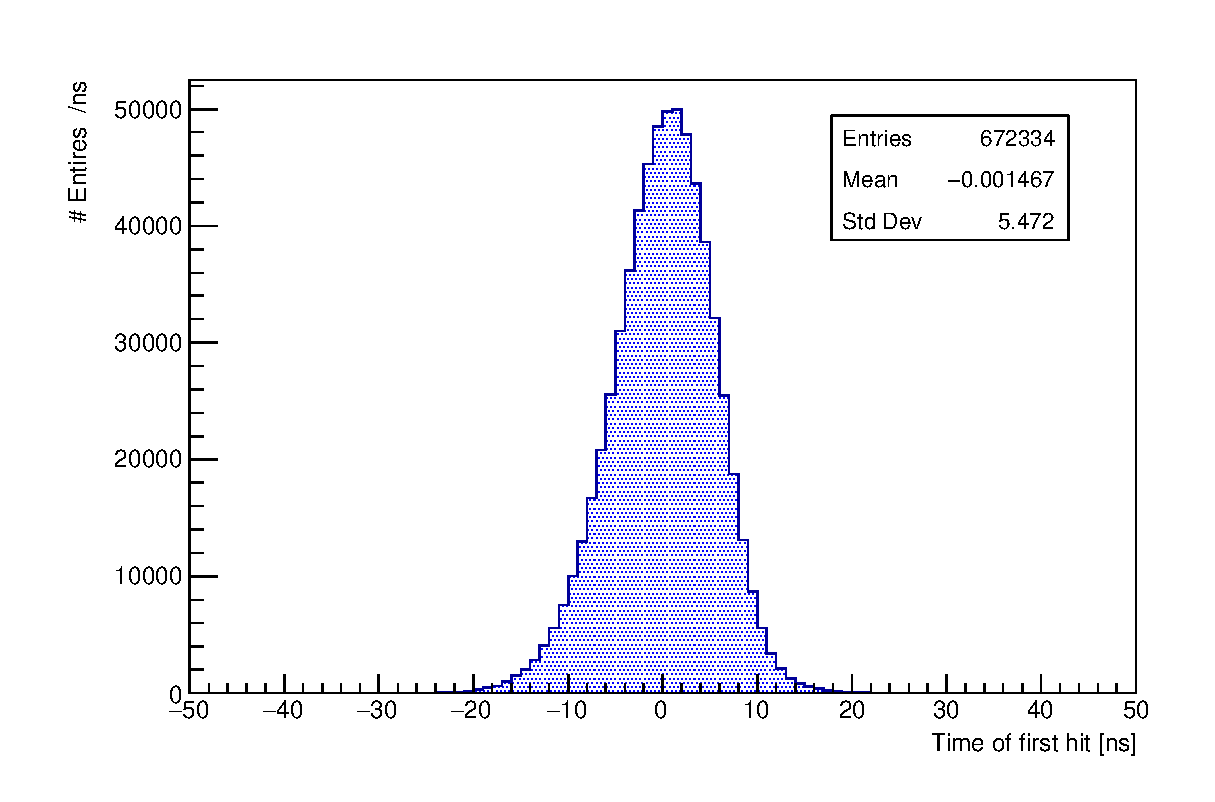
\includegraphics[width=0.5\textwidth]{fig/TimeDistribution_Module3.eps}}
	\caption[]{\textbf{a}: Extracted offset used to correct for mis-calibrations in memory cell pedestals and trigger delay signal. The mean delay of the trigger is $\sim$150 ns. \textbf{b}: Time of the first hit distribution for layer 3. The distribution is clearly asymmetric. $\mu$ = -0.001, RMS = 5.47.}
\end{figure}
The combined time resolution (RMS) obtained by combining all the layer is around 5.85 ns by just applying the time calibration on the data. Some improvements are possible as described in the subsections \ref{subsec:lin_corr} and \ref{subsec:timewalk}.

\subsection{Corrections applied to data}
\subsubsection{Ramp linearity correction}
\label{subsec:lin_corr}

The calibration relies on the linearity of the TDC voltage ramp in the SPIROC2B by measuring the minimum and maximum of the ramp and interpolating assuming a linear ramp. This assumption is not entirely reliable as described in \cite{OskarSSP, EldwanSSP}. For this, a correction of the linearity has to be applied. By simply looking at the time of the first hit (T$_{fH}$) for each chip and BXID versus the TDC value of the hit, the shape of the graph would indicate how reliable is the assumption. Indeed if the ramp would be perfectly linear, one would obtain a flat graph.
A quadratic fit is performed for each chip and BXID in order to correct for the non-linearity of the ramp as shown on figure \ref{fig:LinCorr}. A check has been performed on the quality of the correction, seen on figure \ref{fig:LinCorr_2}.
\begin{figure}[htbp]
	\subfigure[Quadratic fit of chip 188 on layer 12.\label{fig:LinCorr}] 
	{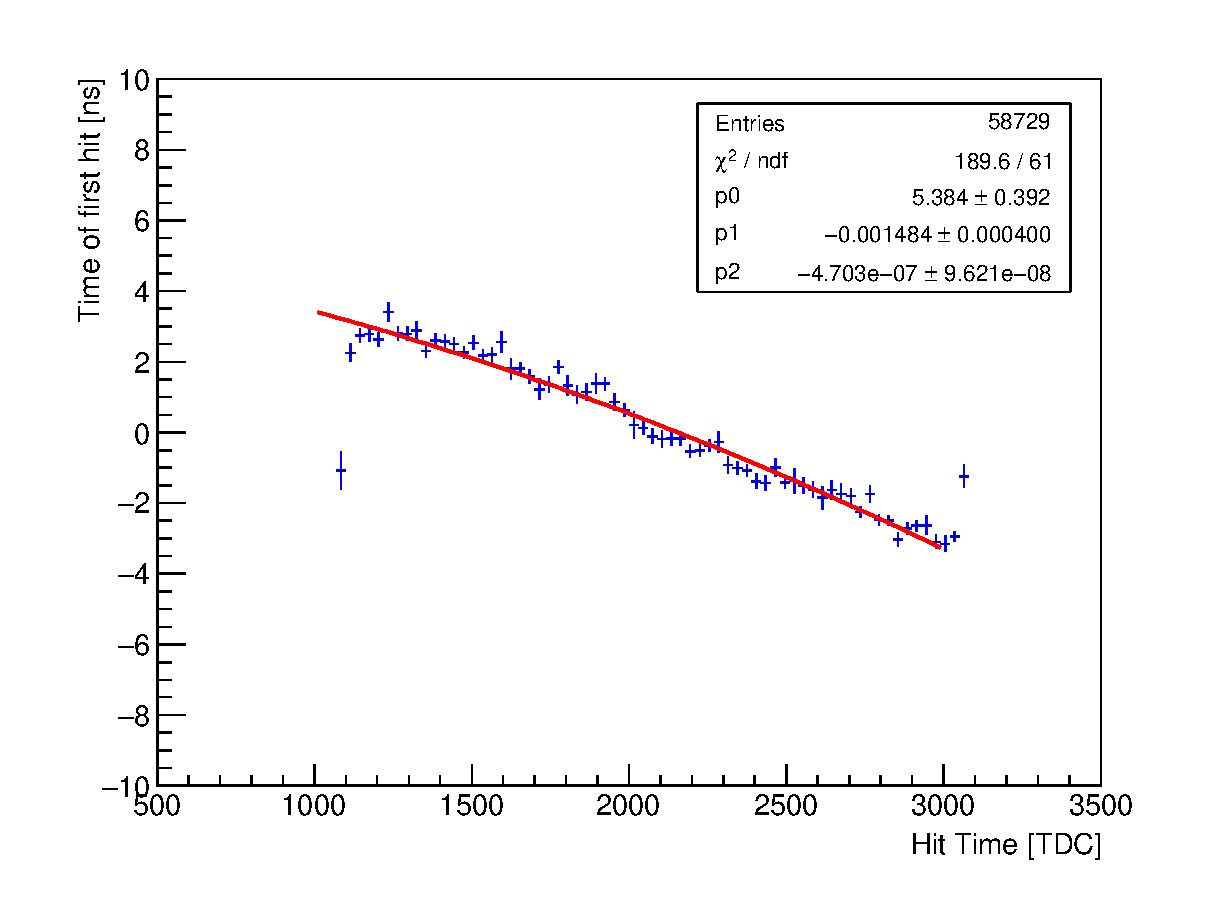
\includegraphics[width=0.5\textwidth]{fig/ProfileFitLinearity.eps}}\hfill
	\subfigure[Profile for chip 188 on layer 12 after the non linearity correction of the ramp.\label{fig:LinCorr_2}]{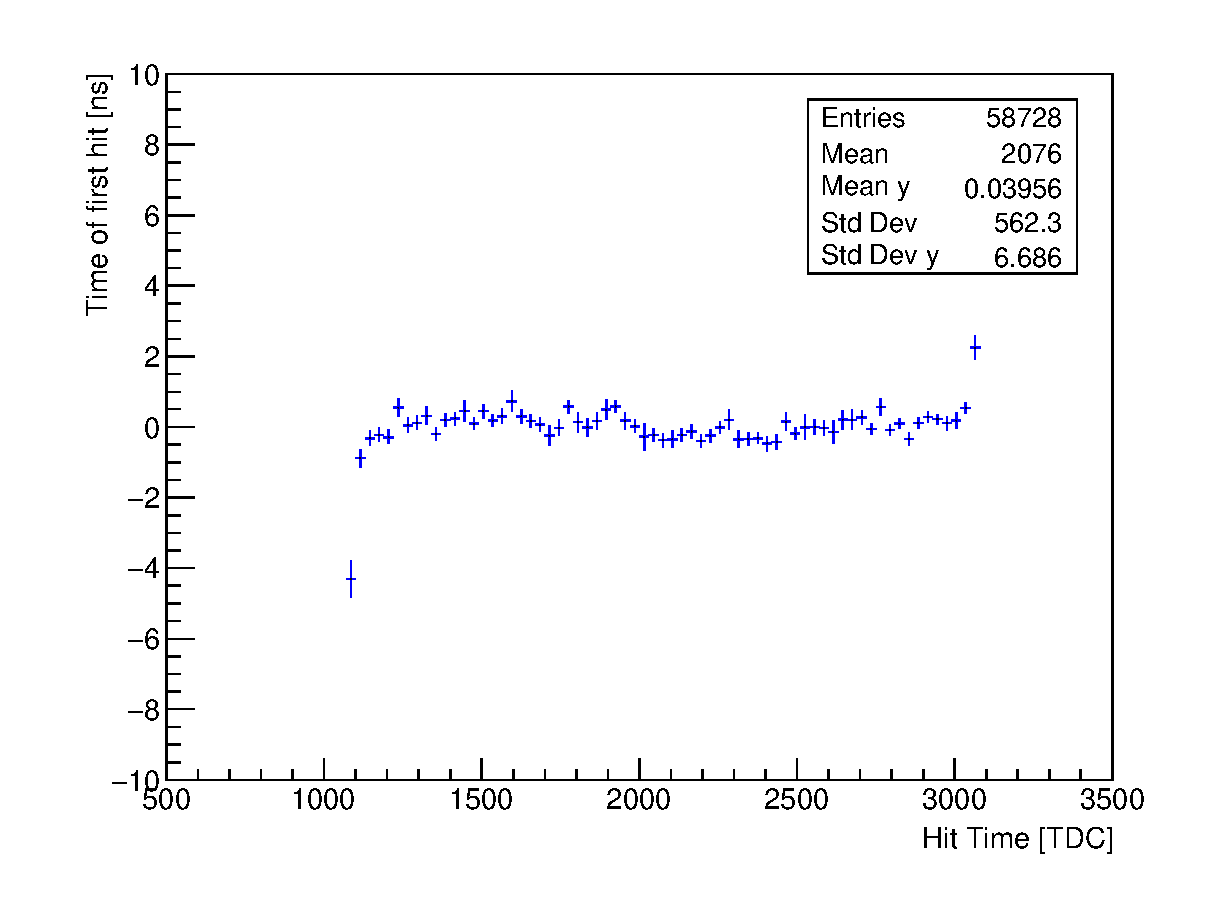
\includegraphics[width=0.5\textwidth]{fig/ProfileFitLinearity_Corr.eps}}
	\caption[]{\textbf{a}: The $\chi^2$ of the fit is to 3.03. \textbf{b}: The correction parameter are applied then on the data to cross-check the quality of the correction. One can see that the curve flattens with the correction applied.}
\end{figure}
The non-linearity correction results in an improvement on the timing resolution of the AHCAL of $\sim$8.2\% (RMS 5.37 ns).

\subsubsection{Time Walk correction}
\label{subsec:timewalk}

The time-walk effect is due to the presence of a threshold that induce a time jitter between a small amplitude signal (under 2 MIP) and a high amplitude signal (more than 2 MIP). Small amplitude signals will systematically trigger at later time than high amplitude signals. %as shown on figure \ref{fig:time_walk_schematics}.
%\begin{figure}[htbp]
%\begin{center}
%\includegraphics[width=0.4\textwidth]{fig/time_walk_effect.png}
%\caption{Time walk effect due to the threshold disriminator. The time registered (t$_A$) for the blue signal (high amplitudes) will be slightly before the time registered (t$_B$) for the red signal (small amplitudes).}
%\label{fig:time_walk_schematics}
%\end{center}
%\end{figure}
A correction can be applied on the data by looking at the time of the first hit versus the amplitude of the hit. This correction mostly applies for low amplitude signals that would widen the time of the first hit distribution, this might be particularly important for late neutrons signals that generally deposit very few energy in the calorimeter.\\
The correction is assumed to be the same for all the chips, independent of the position of the threshold of each chip, as hits are cut at 0.5 MIP and most of the chips were having the threshold set-up well below 0.5 MIP. An exponential fit of the form $\text{A} \times e^{-\lambda{}x} + \text{B}$ is performed on the data to extract the parameters needed to correct the time walk effect.
\begin{figure}[htbp]
	\subfigure[Profile of the time of first hit as function of the hit energy.\label{fig:time_walk_corr}] {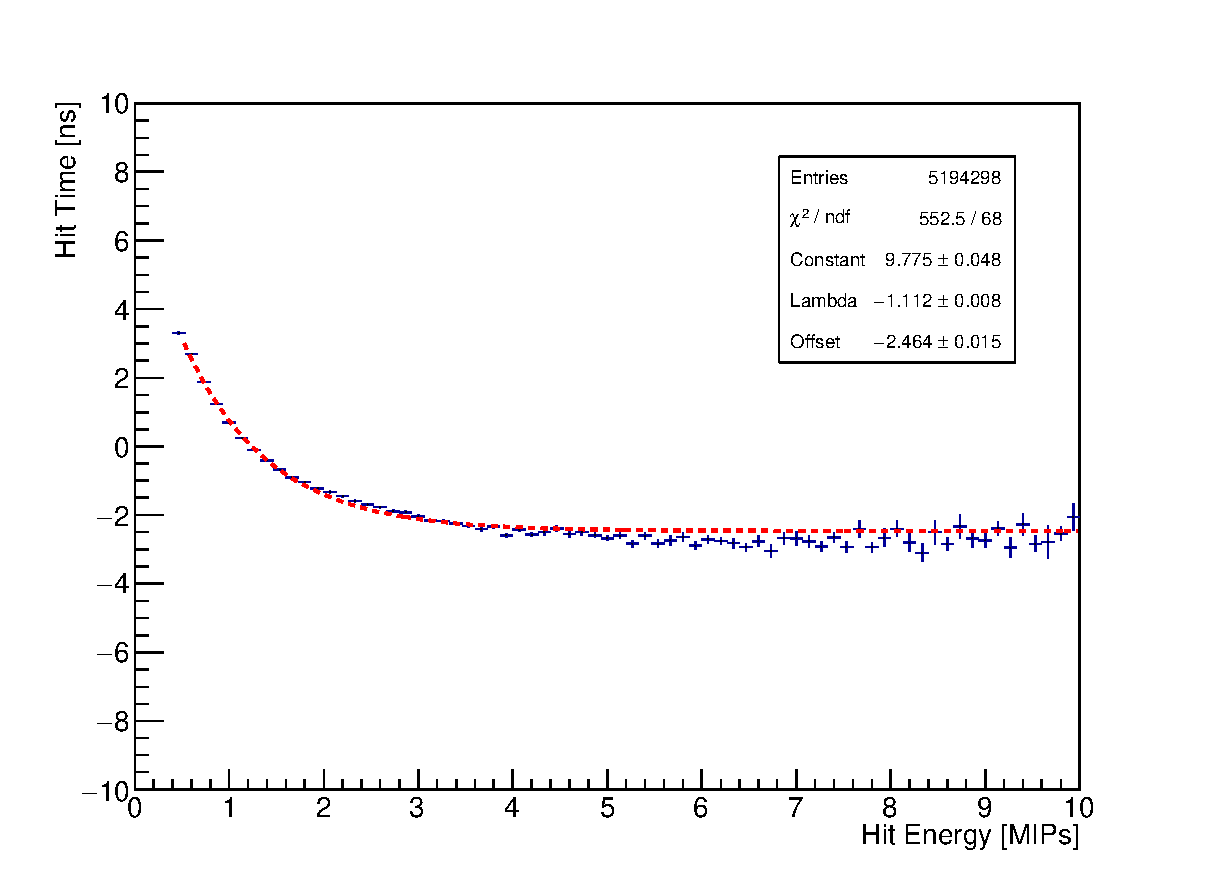
\includegraphics[width=0.5\textwidth]{fig/TimeWalkProfile.eps}}\hfill
	\subfigure[Time of the first hit distribution for layer 3.\label{fig:layer3_time_corr}] {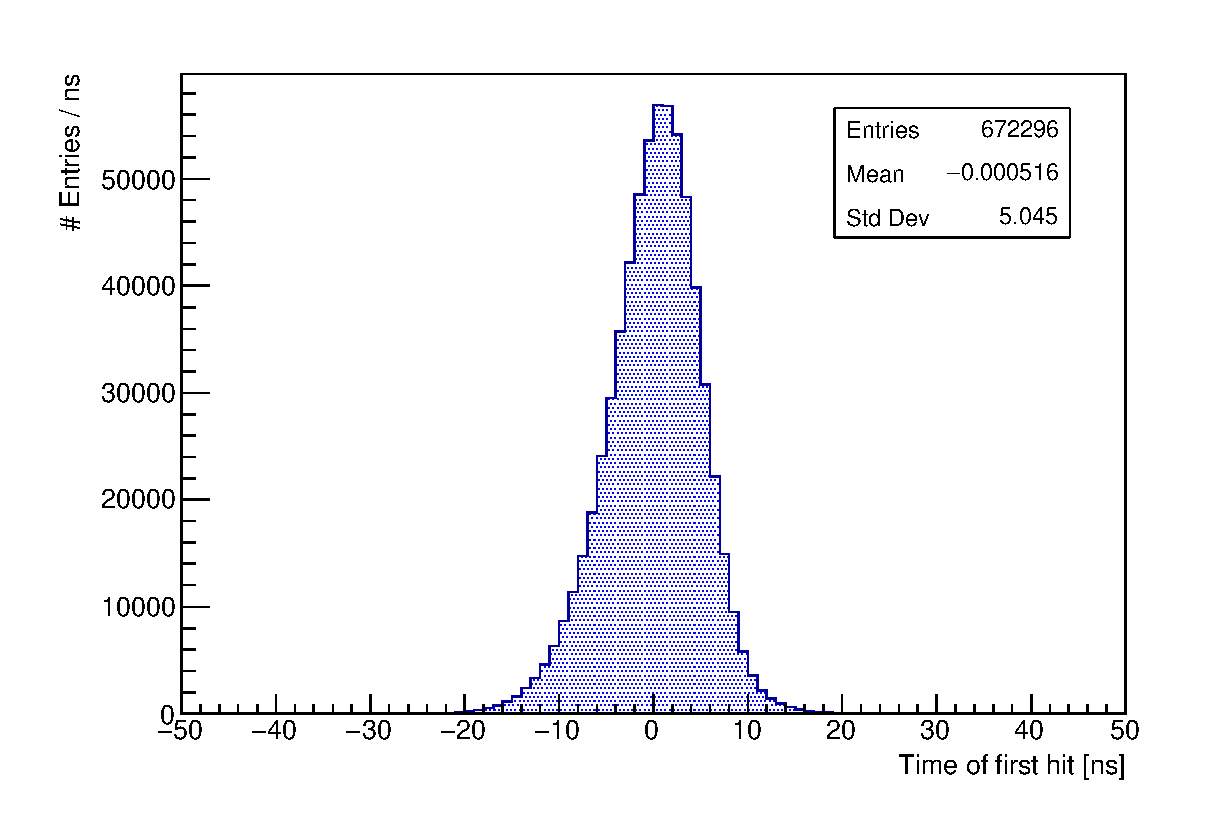
\includegraphics[width=0.5\textwidth]{fig/TimeDistribution_Module3_All.eps}}
	\caption[]{\textbf{a}: Time walk correction extracted from data. A = 9.78 $\pm$ 0.05, $\lambda$ = 1.11 $\pm$ 0.01, B = -2.46 $\pm$ 0.02. A correction up to 4 ns can be applied to low amplitude signals. \textbf{b}: Time of the first hit distribution for layer 3 after all the corrections applied. An improvement of $\sim$8\% is done on the timing resolution for this layer. $\mu$ = -0.001, RMS = 5.05.}
\end{figure}
A maximum improvement of $\sim$15\% can be achieved on the time resolution of the AHCAL for muons (RMS 5.01 ns) as shown on figure \ref{fig:timing_muons}.
\begin{figure}[htbp]
\begin{center}
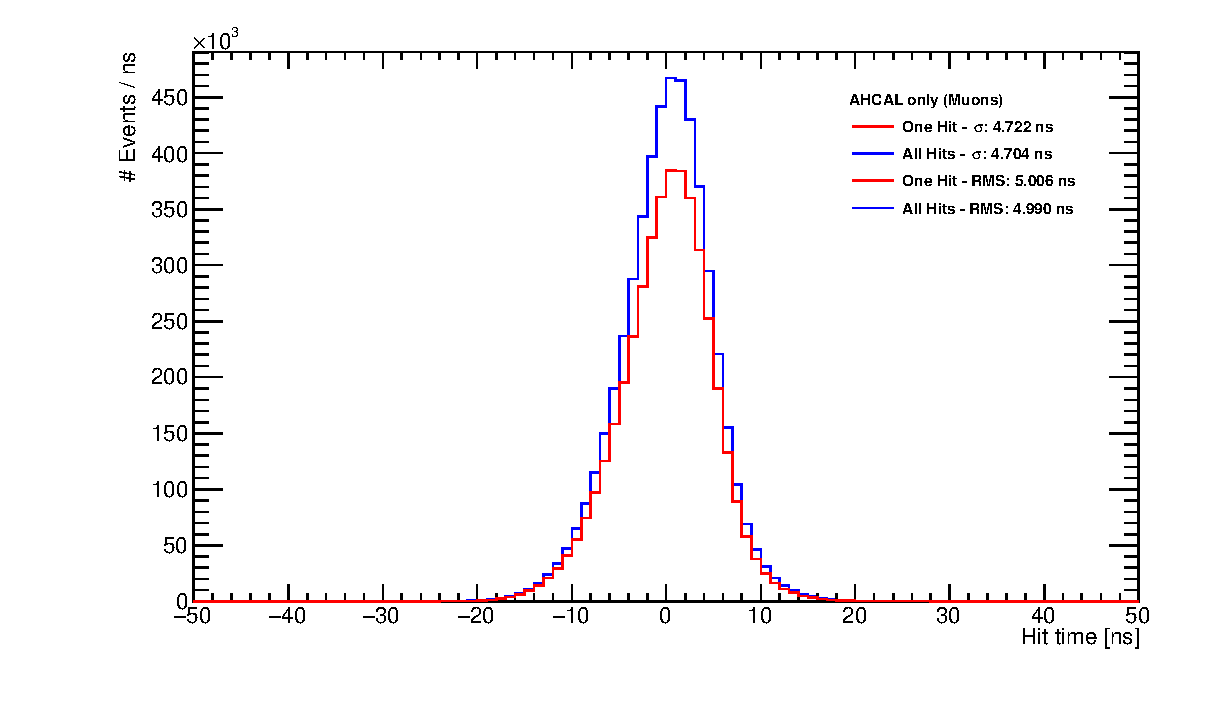
\includegraphics[width=0.6\textwidth]{fig/timing_muons.eps}
\caption{Time of the first hit distribution of the AHCAL after combining all layers and all corrections applied. The red distribution considers only track with single hit per layer. The blue distribution take into account all the hits from muon tracks. RMS$_{\text{One Hit}}$ = 5.00, RMS$_{\text{All Hits}}$ = 4.99.}
\label{fig:timing_muons}
\end{center}
\end{figure}
\subsection{Validation of the calibration}
\label{subsec:validation}

In order to validate the calibration, an electron sample is taken. Electromagnetic showers are quasi-instantaneous and perfect to cross-check the time calibration procedure. The selection applied to the data sample is described in subsection \ref{subsec:elec_sel}. The same calibration constants and correction constants are applied to the data except that an additional offset from the trigger signal has to be corrected for. The additional offset is expected to be small as the trigger configuration is very similar to the one for muons. The figure \ref{fig:delay_elec} shows the offset distribution extracted from data. The mean offset is in the order of 8 ns which seems coherent with the trigger configuration. However, a tail is present in the distribution and it has been related to some chips having problems that is described in the next subsection \ref{subsec:ped_shift}. The data provided by theses chips is ignored in the following analysis.
\begin{figure}[htbp]
	\subfigure[Distribution of trigger delay offset for electrons.\label{fig:delay_elec}] {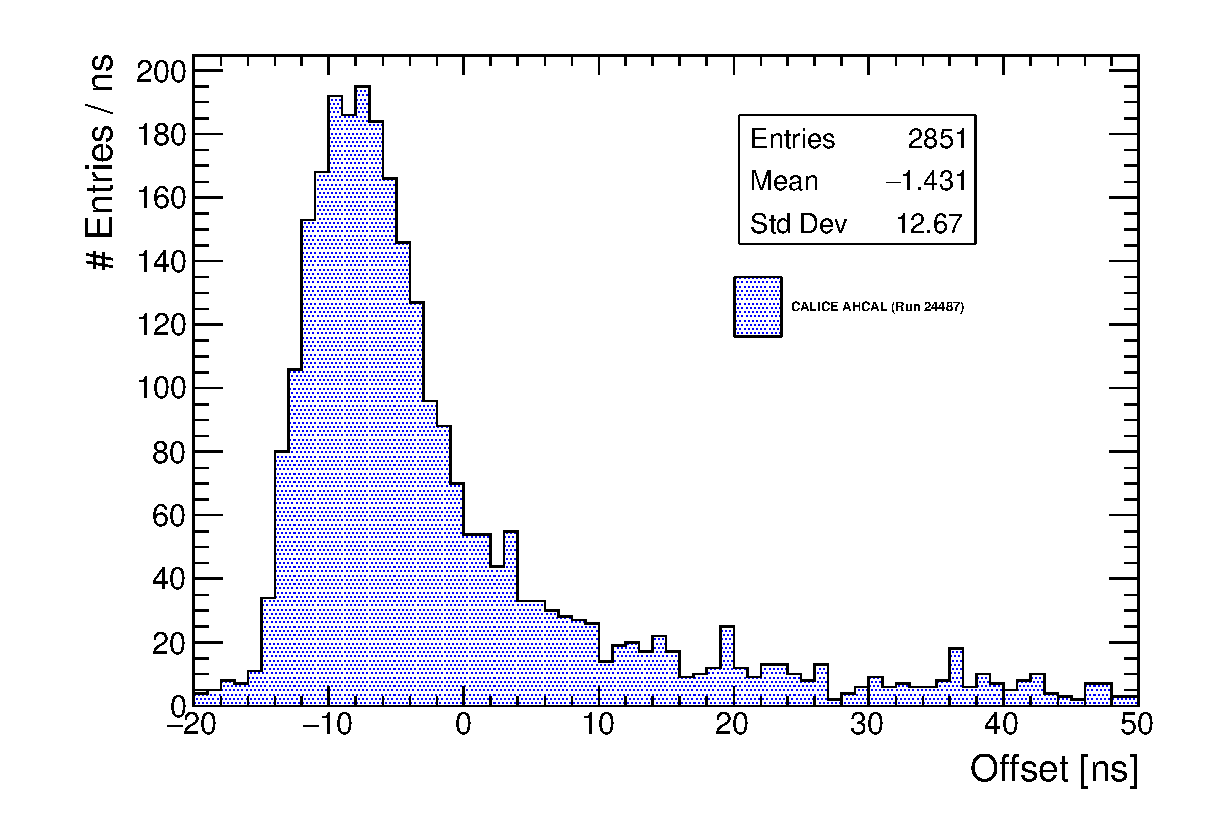
\includegraphics[width=0.5\textwidth]{fig/FittedOffsets_electrons.eps}}\hfill
	\subfigure[Time of the first hit distribution with 20 GeV electrons for the AHCAL.\label{fig:Timing_electrons}] {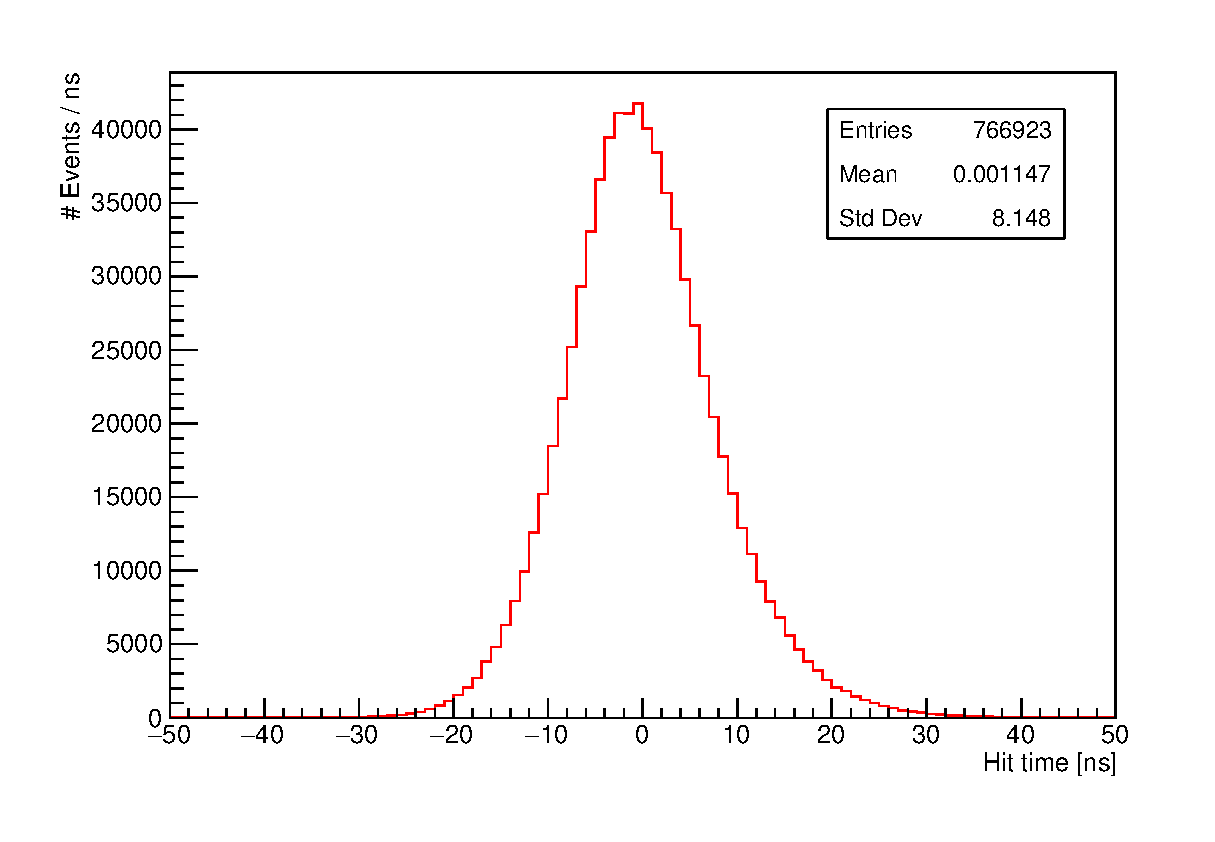
\includegraphics[width=0.5\textwidth]{fig/timing_electrons.eps}}
	\caption[]{\textbf{a}: Distribution of the offset relative to \textit{t=0} for each channel and memory cell. The tail is explained by some chips having problems due to a huge charge inducing a shift of the ground in the chip as explained in subsection \ref{subsec:ped_shift}. \textbf{b}: Time of the first hit distribution for 20 GeV electrons, $\mu$ = 0.001, RMS = 8.15.}
\end{figure}
Once the offset is corrected, the time of the first hit can be determined for each channel seen in figure \ref{fig:Timing_electrons}. The distribution presents a large tail to the right and moreover is much wider than for muons. This gives a hint that an effect is present in electron data but not in muon data. The difference seen could be related to the fact that in electromagnetic showers, the number of hits is much higher as well as the energy deposited in a single cell can be over hundreds MIP. This effect has been investigated in the next subsection. 

\subsection{Pedestal shift effect}
\label{subsec:ped_shift}

Pedestal shift for energy measurement is not a new feature of the SPIROC2B chip and is still intensively investigated \cite{OskarMaster}. The effect comes certainly from the fact that a ground shift occurs in the chip when a saturated signal is present in a certain amount of channels. As well it may induced a shift of the trigger threshold and thus can have an impact on the time of the hit. This effect can be investigated by looking at the time of the first hit function of the number of triggered channels. This has been done as shown in figure \ref{fig:nhits_profile}.
\begin{figure}[htbp]
\begin{center}
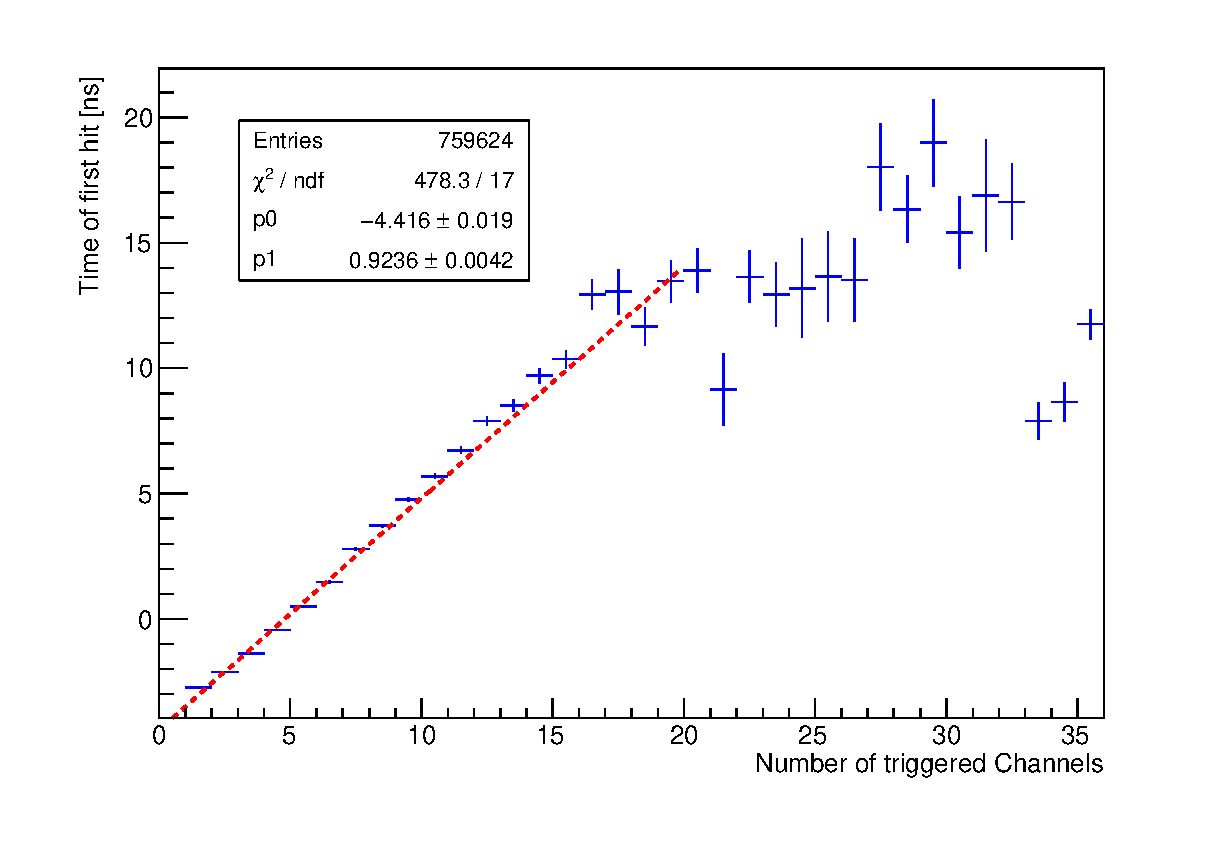
\includegraphics[width=0.6\textwidth]{fig/TimeHits_NumberTriggeredChn_Dep.eps}
\caption{Time of the first hit function of the number of triggered channels in a chip. The fit region is between 1 and 20 hits. A linear dependence seems to be visible.}
\label{fig:nhits_profile}
\end{center}
\end{figure}
The pedestal shift can have a drastic effect on the time resolution of the AHCAL, a correction up to 15 ns can be necessary to the data for a high number of trigger. Moreover, the correction might be dependent for each chip but this has not been investigated at the moment.\\
Once the parameters for the correction have been determined, it is applied to the electron data sample and the distribution of the time of the first is again shown in figure \ref{fig:timing_electrons_corr}.
\begin{figure}[htbp]
\begin{center}
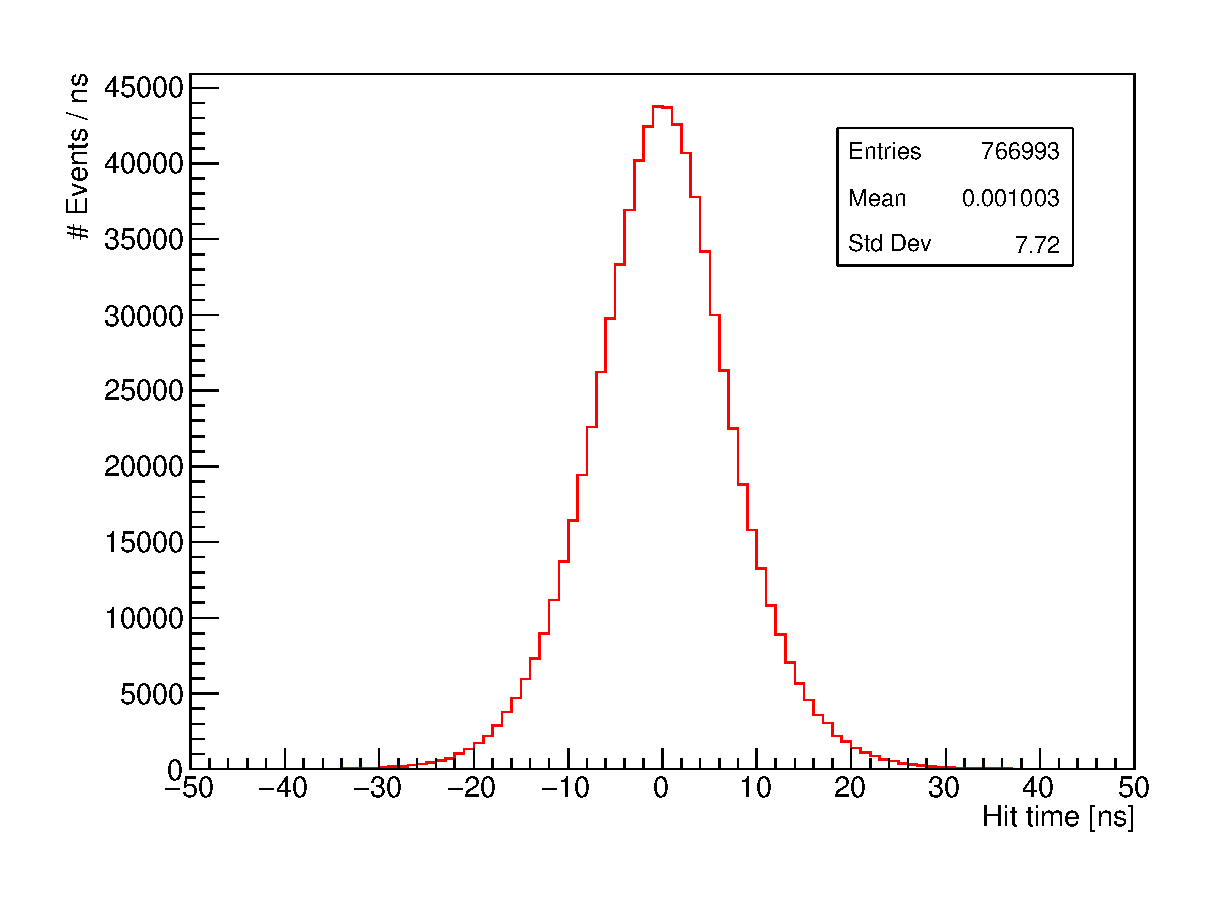
\includegraphics[width=0.6\textwidth]{fig/timing_electrons_corr.eps}
\caption{Time of the first hit distribution for 20 GeV electrons after number of triggered channel correction, $\mu$ = 0.001, RMS = 7.72.}
\label{fig:timing_electrons_corr}
\end{center}
\end{figure}
As expected the correction improves the RMS of the distribution ($\sim$5.3\%) as well as the distribution appears more gaussian-like. However, there is still a discrepancy with the time resolution from muons (5.0 ns, $\sim$35.2\% difference). This might indicates that the pedestal shift correction is only a mean correction of the effect thus does not perform perfectly. In order for the simulation to match the data, the increase of the width of the distribution has to be parametrised somehow. More details can be read in the appendix \ref{appendix:ped_shift}.

\subsection{Comparison with Simulation}

The next step is to compare data with simulation and validate the simulation with electrons. The timing resolution is extracted from muon data runs for each layer by fitting a gaussian in the range [-50 ns, 50 ns] and is used to smear the timing of simulated hits. The table \ref{table:time_res_sim} sums up the resolution used.
\begin{table}[htbp]
\centering
  \begin{tabular}{@{} cc @{}}
    \hline
    Layer & Timing Resolution [ns] \\ 
    \hline
     3 & 4.74 \\ 
     4 & 4.30 \\
     5 & 4.12 \\
	 6 & 5.61 \\
	 7 & 5.51 \\
	 8 & 5.26 \\
    \hline
  \end{tabular}
  \hspace{2ex}
  \begin{tabular}{@{} cc @{}}
    \hline
    Layer & Timing Resolution [ns] \\ 
    \hline
	 9 & 4.70 \\
	 10 & 6.18 \\
	 11 & N/A \footnotemark[1] \\
	 12 & 4.39 \\
	 13 & 4.47 \\
	 14 & 4.38 \\
	\hline
  \end{tabular}
  \caption{Timing resolution extracted with a gaussian fit from muon data used for simulation.}
  \label{table:time_res_sim}
\end{table}
\footnotetext{The chips on this layer have a noisy problem leading to a right tail in the distribution and thus are excluded.} 
The comparison for muons is shown on figure \ref{fig:sim_data_muon}. The pedestal shift correction is not applied as it is supposed to be negligible for muons. Generally 1 or 2 channels can be triggered in the same chip at maximum thus limiting the pedestal shift effect. 
\begin{figure}[htbp]
	\subfigure[Time of first hit for data and simulation between -50 and 50 ns.\label{fig:muon_sim_data_1}] {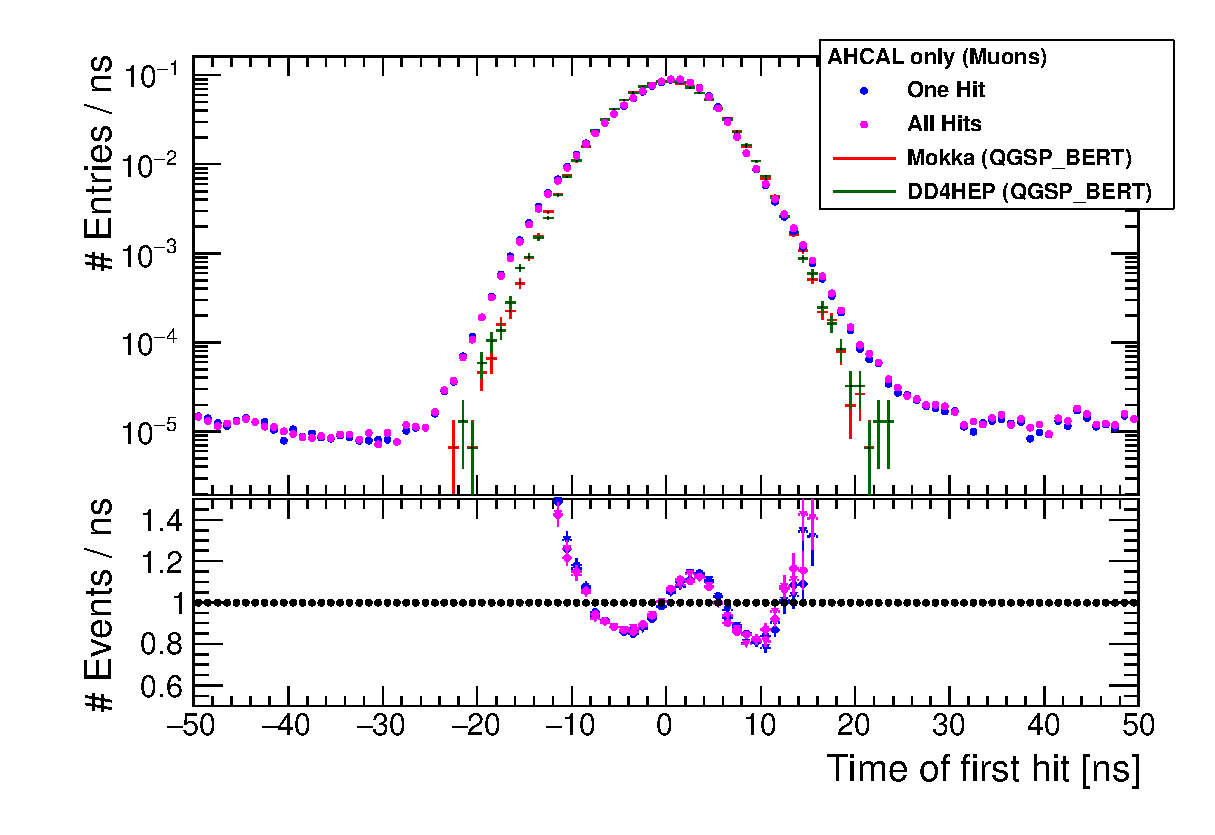
\includegraphics[width=0.5\textwidth]{fig/Comparison_SimData_Muons.eps}}\hfill
	\subfigure[Time of first hit for data and simulation zoomed between 1 and 200 ns.\label{fig:muon_sim_data_2}] {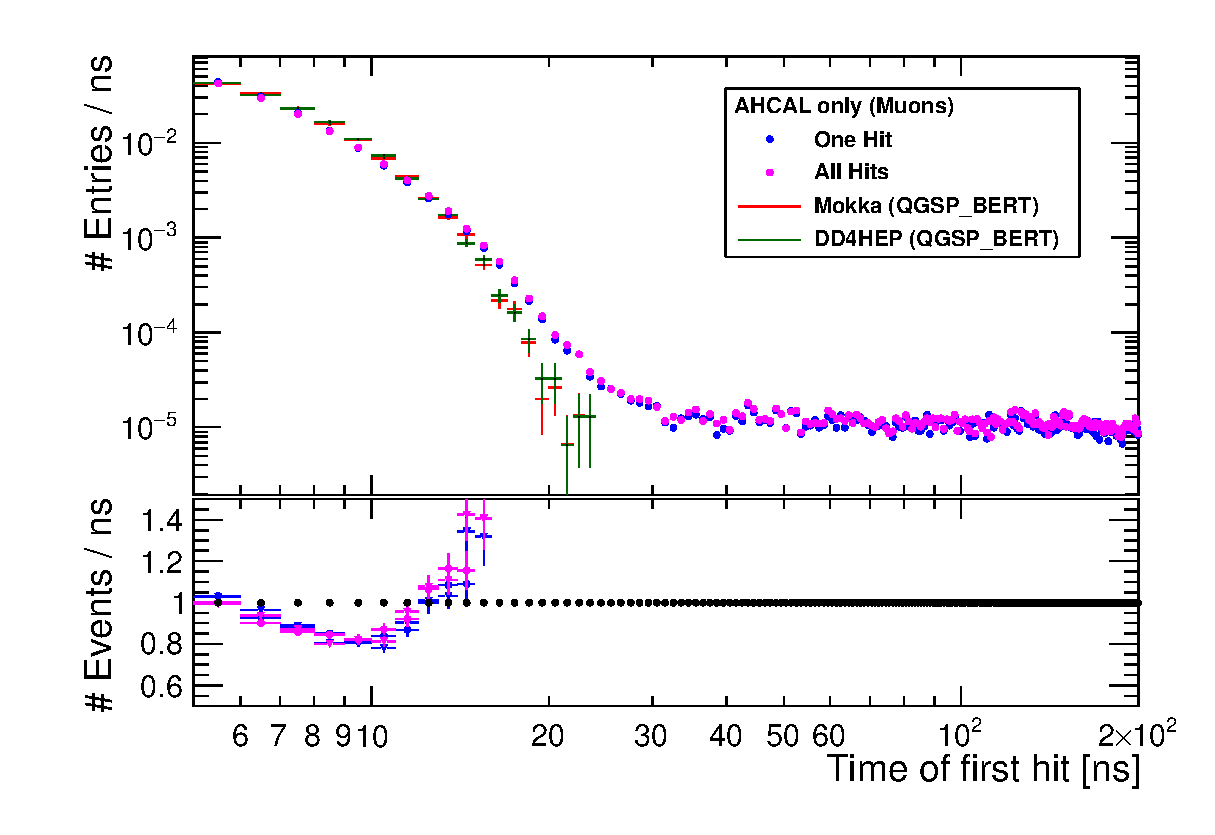
\includegraphics[width=0.5\textwidth]{fig/Comparison_SimData_Muons_zoom.eps}}
	\caption[]{\textbf{a}: The simulation matches to the data up to 20\% in the region -10 to 10 ns. \textbf{b}: Zoom in the region 1 to 200 ns, improvements are needed to match data and especially after 20 ns, modelling of the data is missing due to late noise hits.}
	\label{fig:sim_data_muon}
\end{figure}
The comparison shows that in the range [-10, 10] ns, the difference between data and simulation is around 20\% maximum. Under -10 ns, the simulation is much more in disagreement due to the asymmetric shape in data that is not reproduced in simulation. But the most interesting part is the right side of the time distribution. Here, between 10 and 20 ns, the agreement between data and Monte-Carlo worsens. This is certainly because of the tail present in data that is due to late noise events and random delays in the relative trigger signal from the scintillator triggers which is not implemented in Monte-Carlo. Theses distributions show that the simulation performs well in the first tens of nanoseconds but that more work needs to be invested in the reproduction of the data up to 200 ns which is important for hadronic showers.\\
In the next step, a comparison with electron data is necessary to validate the simulation. The time resolution used for each layer is the same shown in table \ref{table:time_res_sim}. The figure \ref{fig:sim_data_elec} shows this comparison.
\begin{figure}[htbp]
	\subfigure[Time of first hit for data and simulation between -50 and 50 ns.\label{fig:elec_sim_data_1}] {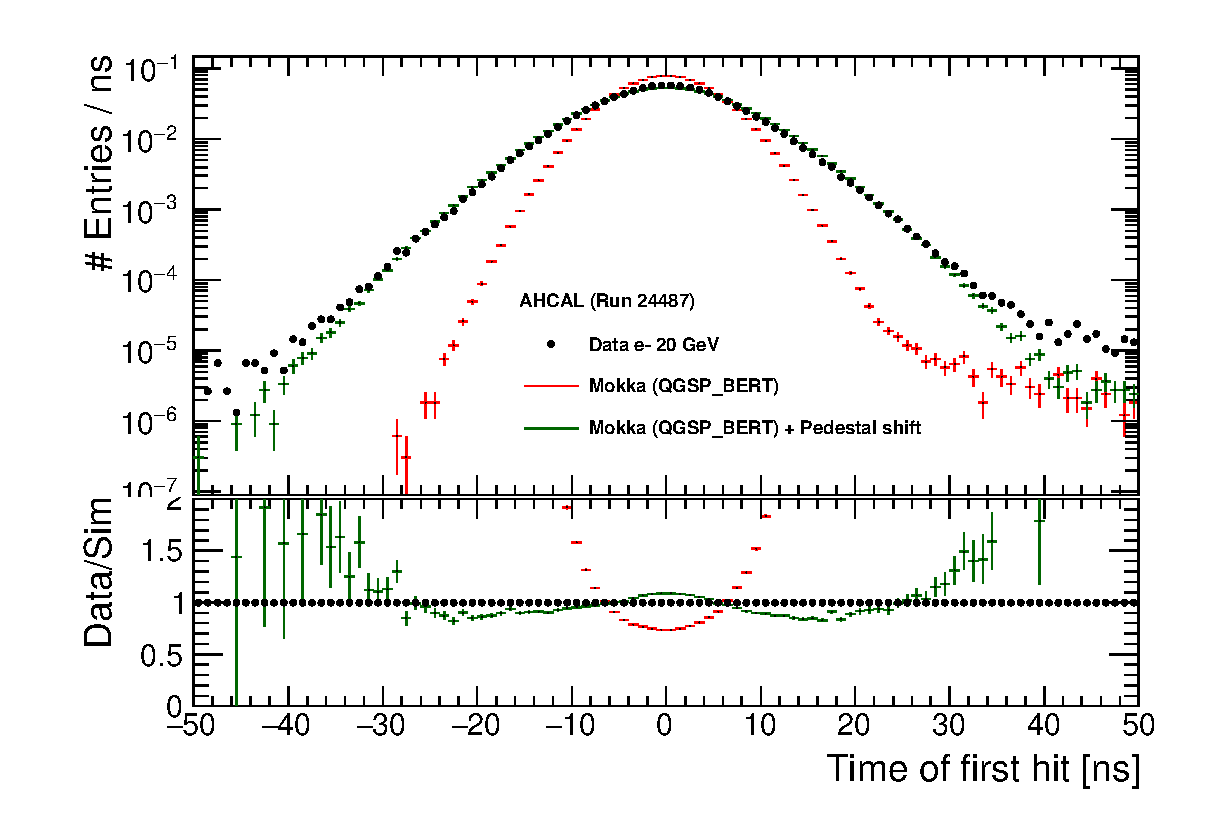
\includegraphics[width=0.5\textwidth]{fig/Comparison_SimData_Electrons_AfterCorrection.eps}}\hfill
	\subfigure[Time of first hit for data and simulation zoomed between 1 and 200 ns.\label{fig:elec_sim_data_2}] {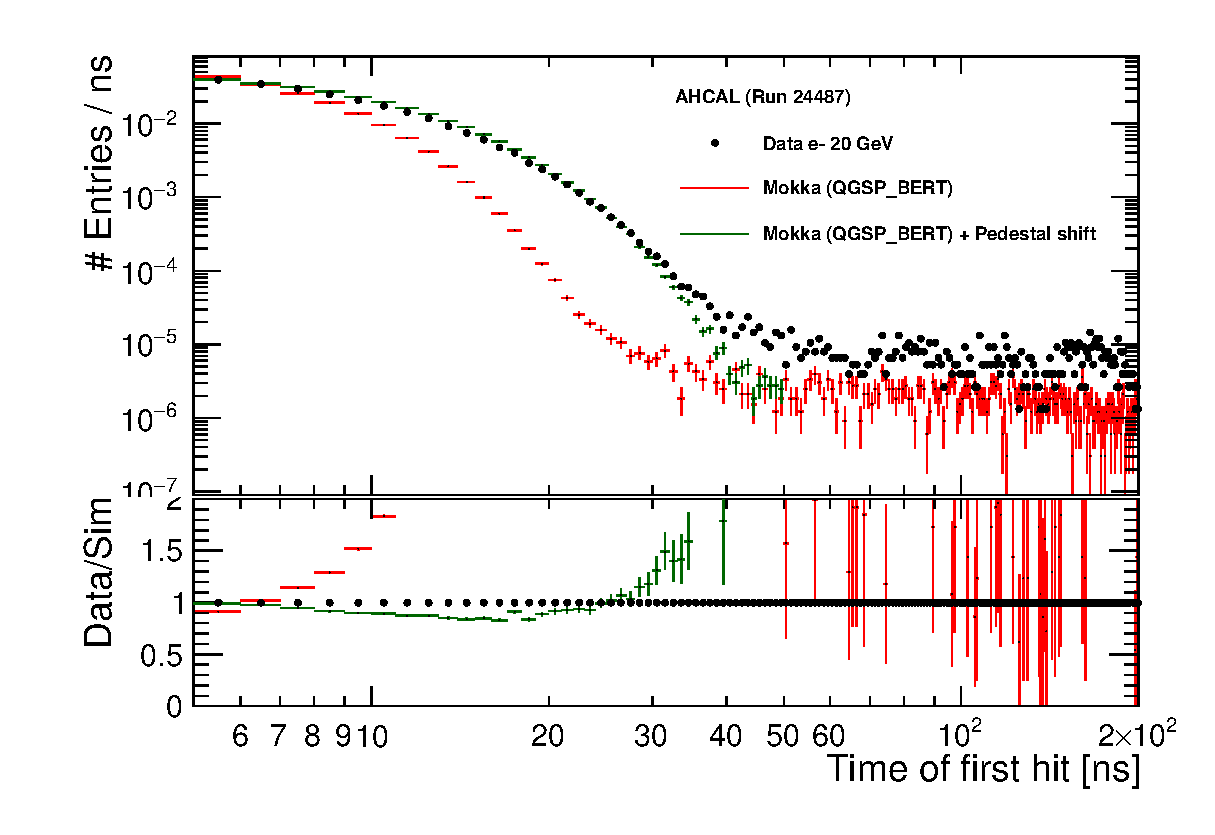
\includegraphics[width=0.5\textwidth]{fig/Comparison_SimData_Electrons_AfterCorrection_zoom.eps}}
	\caption[]{\textbf{a}: The red curve shows the simulation with only the resolution extracted from muons. The green curve is the simulation after the implementation of the pedestal shift in the digitisation. \textbf{b}: The simulation in green shows a good agreement with the data up to 20 ns. The tail after is coming from noise events that is not modelled in the simulation.}
	\label{fig:sim_data_elec}
\end{figure}
As expected, the simulation in red curve does not match the data. This is because of the pedestal shift effect that is still present in data as the correction applied function of the number of triggered channels is only a global correction and not event by event. The right tail present in simulation is caused by small energy depositions from the electromagnetic shower corresponding to a very small fraction of events occurring ($\sim$0.1\%).
After the parametrisation of the pedestal shift effect in simulation as described in appendix \ref{appendix:ped_shift}, the green curve is in much better agreement (up to $\sim$15\%) with the data in the range [-20, 20] ns.

\section{Runs \& Event Selection}
 
During the SPS testbeam in July 2015, $\mu^-$, $e^-$ and $\pi^-$ runs were taken with beam momenta ranging from 10 GeV to 150 GeV. 
The runs and number of events used in this analysis are listed in table \ref{}.

\subsection{Pion Selection}

To be done!

\section{Results}

To be done!

\section{Summary}

\clearpage

\addcontentsline{toc}{section}{Bibliography}
\begin{thebibliography}{10}

\bibitem{SPSBeamLine}
	CERN, \textit{Secondary Beam \& Areas}, \\
	http://sba.web.cern.ch/sba/BeamsAndAreas/h2/H2manual.html
\bibitem{CAN-038}
	The CALICE Collaboration, \textit{The Time Structure of Hadronic Showers in Tungsten and Steel with T3B}, \\
	CALICE Analysis Note CAN-038
\bibitem{OskarSSP}
	 O. Hartbrich, \textit{Investigation of the time measurement capabilities of the SPIROC2b ASIC}, \\
	 DESY summer student report, 2011.
\bibitem{EldwanSSP}
	 E. Brianne, \textit{Studies of the front-end electronics of the Analog HCAL}, \\
	 DESY summer student report, 2012.
\bibitem{OskarMaster}
	 O. Hartbrich, \textit{Commissioning and LED System Tests of the Engineering Prototype of the Analog Hadronic Calorimeter of the CALICE Collaboration}, \\
	 DESY-thesis-2012-040, ISSN 1435-8085.
\bibitem{CAN-002} 
	 The CALICE Collaboration, \textit{First results from electron data with the CALICE tile HCAL prototype at the CERN test-beam}, \\
	 CALICE Analysis Note CAN-002
\bibitem{CAN-010} 
	 The CALICE Collaboration, \textit{Electron data with the CALICE tile AHCAL prototype at the CERN test-beam - Update}, \\
	 CALICE Analysis Note CAN-010
\bibitem{JINST-6}
	 The CALICE Collaboration, C. Adloff et al., \textit{Electromagnetic response of a highly granular hadronic calorimeter}, \\
	 2011 JINST 6 P04003, doi:10.1088/1748-0221/6/04/P04003
\bibitem{DAQ}
	 T. Suehara et al., \textit{AIDA-CALICE DAQ interface} \\
	 AIDA 2020 Scientific/Technical Note, AIDA-2020-NOTE-2016-006
\end{thebibliography}

\clearpage
\begin{appendix}
\section*{Appendix}
\pagestyle{plain}
%\setcounter{table}{0}
\renewcommand{\thetable}{A\arabic{table}}
\addcontentsline{toc}{section}{Appendix}
\addtocontents{toc}{\protect\setcounter{tocdepth}{0}}

\section{Error Estimation of the TDC calibration.}
\label{appendix:calib_error}

In this appendix, a small study of the error made on the calibration from TDC to nanoseconds is done. By simple calculation, the conversion is done is the following way:
\begin{equation*}
\begin{split}
\text{T} \: \text{[ns]} & = ( \text{TDC} - \text{Ped} ) * \text{slope} \\
& = ( \text{TDC} - \text{Ped} ) * \frac{\text{A}}{(\text{Max} - \text{Ped})} \quad \text{with A = 3920 ns}
\end{split}
\end{equation*}
To avoid correlations between the slope and the pedestal, the error is obtained by differentiating w.r.t Max and Ped. The error is then obtained via:
\begin{equation*}
\partial t^2 = \left(\frac{\partial t}{\partial Ped}\right)^2 \times \sigma_{Ped}^2 + \left(\frac{\partial t}{\partial Max}\right)^2 \times \sigma_{Max}^2 + \left(\frac{\partial t}{\partial A}\right)^2 \times \sigma_{A}^2
\end{equation*}
Assuming that $\sigma_{A}$ is null, we get the following formula:
\begin{equation*}
\partial t^2 = \frac{1}{(\text{Max} - \text{Ped})^2} \left[ \left( \frac{\text{A(TDC - Max)}}{(\text{Max} - \text{Ped})} \right)^2 \times \sigma_{Ped}^2 + \left( \frac{\text{A(TDC - Ped)}}{(\text{Max} - \text{Ped})} \right)^2 \times \sigma_{Max}^2 \right]
\end{equation*}
As one can expect, the formula is symmetric and should be minimum in the middle of the ramp as long as $\sigma_{Max}$ and $\sigma_{Ped}$ are similar. On the other hand, the error will be greater on one side or the other depending on tcdhe $\sigma$ being the biggest. 
\begin{figure}[htbp]
	\subfigure[Errors extracted from the edge detection for the pedestal for each chip. channel, memory-cell and BXID.\label{fig:error_ped}] {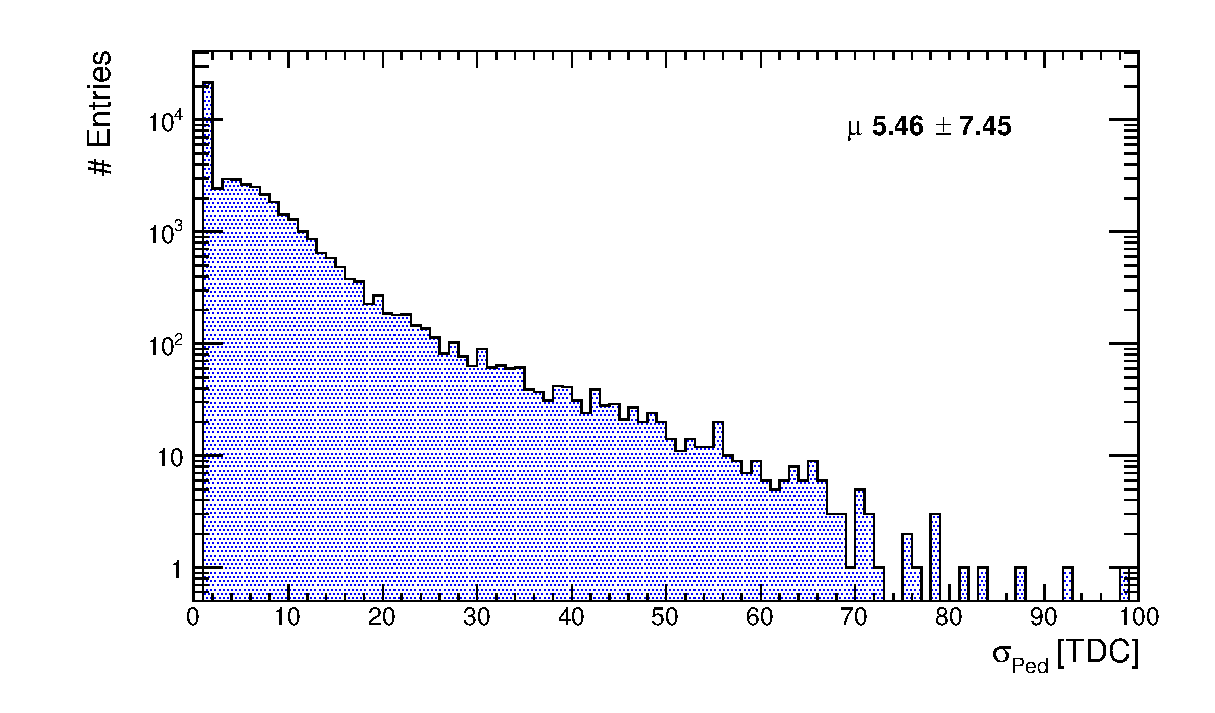
\includegraphics[width=0.5\textwidth]{fig/PedestalErrorDistribution_AHCAL.eps}}\hfill
	\subfigure[Error extracted from the edge detection for the maximum of the ramp for each chip and BXID.\label{fig:error_max}] {\includegraphics[width=0.5\textwidth]{fig/ErrorMaxDistribution.eps}}
	\caption[]{\textbf{a}: Pedestal error distribution extracted for all channels in the detector, most of the errors made are small with a high tail certainly due to the limited statistics for some channels and memory-cells. $\mu$ = 5.46 TDC, RMS = 7.45 TDC \textbf{b}: Maximum error distribution extracted from the edge detection method for each chip and BXID. The error is a bit higher than for the pedestal due to the difficulty to detect perfectly the end of the ramp. $\mu$ = 9.71 TDC, RMS = 4.90 TDC.}
	\label{fig:error_dist}
\end{figure}
The errors estimations $\sigma_{Max}$ and $\sigma_{Ped}$ are described in subsection \ref{subsec:slope_calib}. Distributions of the errors extracted can be seen on figures \ref{fig:error_ped} and \ref{fig:error_max}. Theses errors are obtained arbitrary due to the threshold variation and are likely to be over-estimated as they are not reflected in the final timing distribution. Moreover, the shift of the distribution to zero is correcting the error made on the pedestal for each channels thus $\sigma_{Ped}$ is likely to be null. 
\begin{figure}[htbp]
	\subfigure[Calibration error made on the conversion to nanosecond for a channel on layer 3.\label{fig:error_chn}] {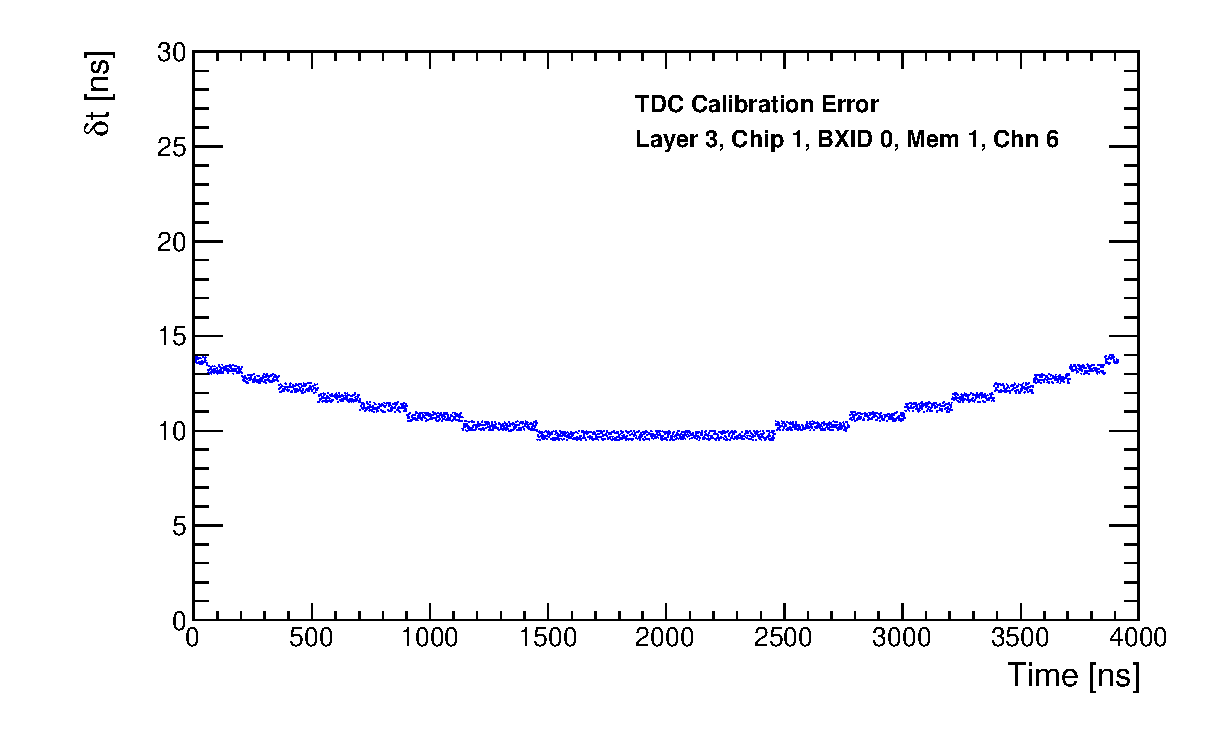
\includegraphics[width=0.5\textwidth]{fig/TimeErrorEstimation_Layer3.eps}}\hfill
	\subfigure[Calibration error made on the conversion to nanosecond for a channel on layer 5.\label{fig:error_chn2}] {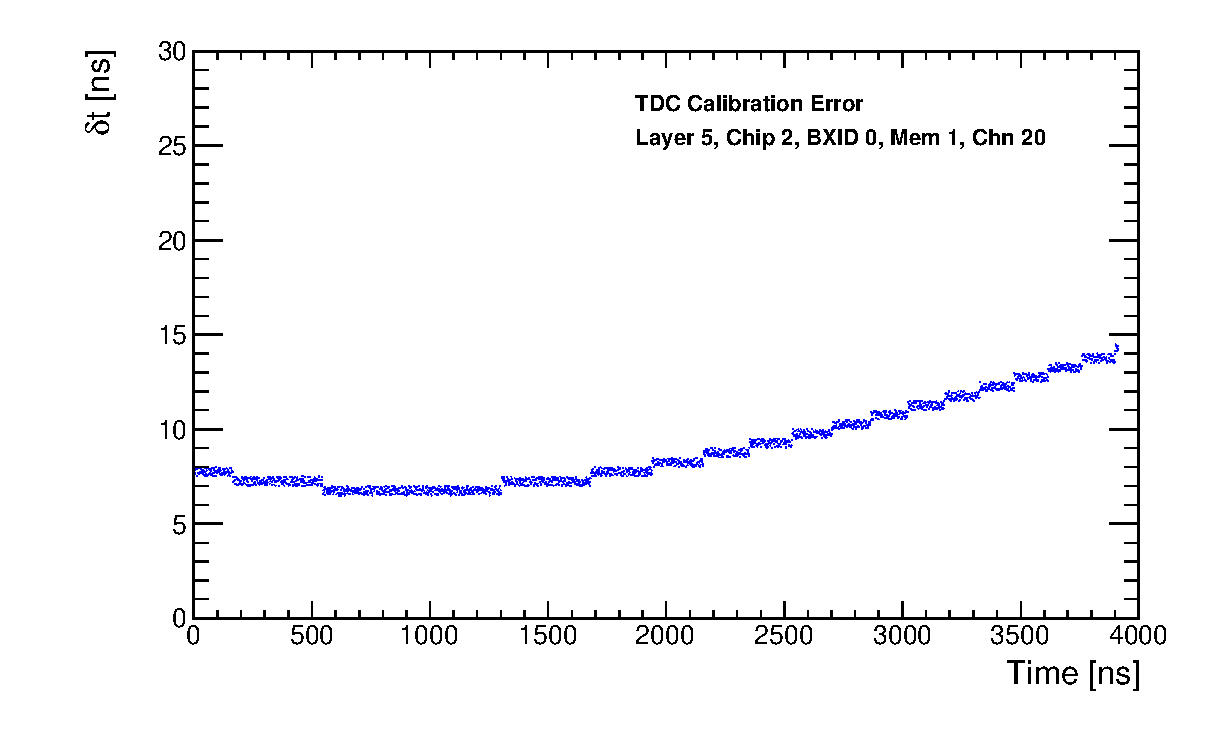
\includegraphics[width=0.5\textwidth]{fig/TimeErrorEstimation_Layer5.eps}}
	\caption[]{\textbf{a}: Error distribution made for a single channel on layer 3. The error is variating between 10 and 14 ns but is likely to be over-estimated and not valid for the final time distribution. \textbf{b}: Error distribution made for a single channel on layer 5. The error is variating between 7 and 14 ns but is likely to be over-estimated and not valid for the final time distribution.}
	\label{fig:error_calibration}
\end{figure}
The figure \ref{fig:error_chn} represent the error made for one channel selected in a single chip for a single memory cell and BXID. It shows the symmetric behaviour of the error and present a minimum around the middle of the ramp. This not a typical channel as mostly the maximum has an error higher than the pedestal due to the difficulty to pick perfectly the maximum of the ramp with the sharp falling edge. A more typical channel can be seen on figure \ref{fig:error_chn2}.
The estimated error made on the calibration from TDC to nanoseconds is around 1-2 ns.

\newpage
\section{Pedestal shift study and parametrisation in Monte-Carlo.}
\label{appendix:ped_shift}

The correction applied function of the number of hits is only a global correction not an event to event basis correction. Thus a part of the pedestal shift effect remains or it could be another effect from the electronics that is not yet identified.\\
This effect has to be implemented in the simulation in order to match the timing distribution of electrons without also influencing the time distribution for muons. A parametrisation is thus implemented in the Monte-Carlo extracted from data. This parametrisation assumes the following, the effect is additional to the seen muon resolution giving then:
\begin{equation*}
\begin{split}
& \sigma_{\text{obs}}^2 = \sigma_{\mu}^2 + \sigma_{\text{PedShift}}^2 \\
& \Leftrightarrow \sigma_{\text{PedShift}} = \sqrt{\sigma_{\text{obs}}^2 - \sigma_{\mu}^2}
\end{split}
\end{equation*}
The $\sigma_{\text{PedShift}}$ is then extracted from data by fitting with a gaussian the timing distribution obtained for each bin in number of triggered channels in a chip as shown in figure \ref{fig:ped_shift_dist_para}. By plotting the gaussian width extracted function of the number of triggered channels in a chip, one can extract the parametrisation of the effect. The figure \ref{fig:para_fit} is fitted with a function in the shape:
\begin{equation*}
\sigma_{\text{PedShift}} = A \times ( 1 - e^{-\frac{\epsilon x}{A}} ) + \alpha \times x
\end{equation*}
\begin{figure}[htbp]
	\subfigure[Time of the first hit distribution for different binning of number of triggered channels in a chip.\label{fig:ped_shift_dist_para}] {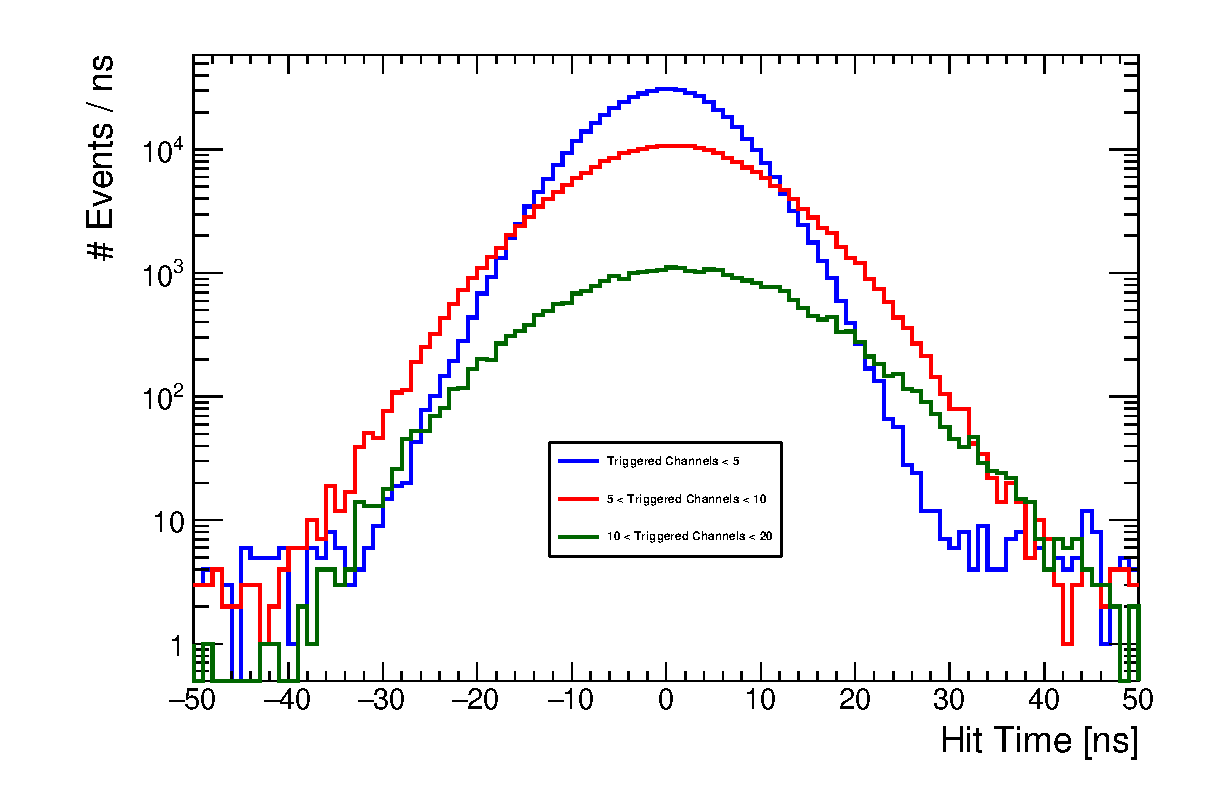
\includegraphics[width=0.5\textwidth]{fig/TimingnHitsBins.eps}}\hfill
	\subfigure[Gaussian width extracted function of the number of triggered channels in a chip.\label{fig:para_fit}] {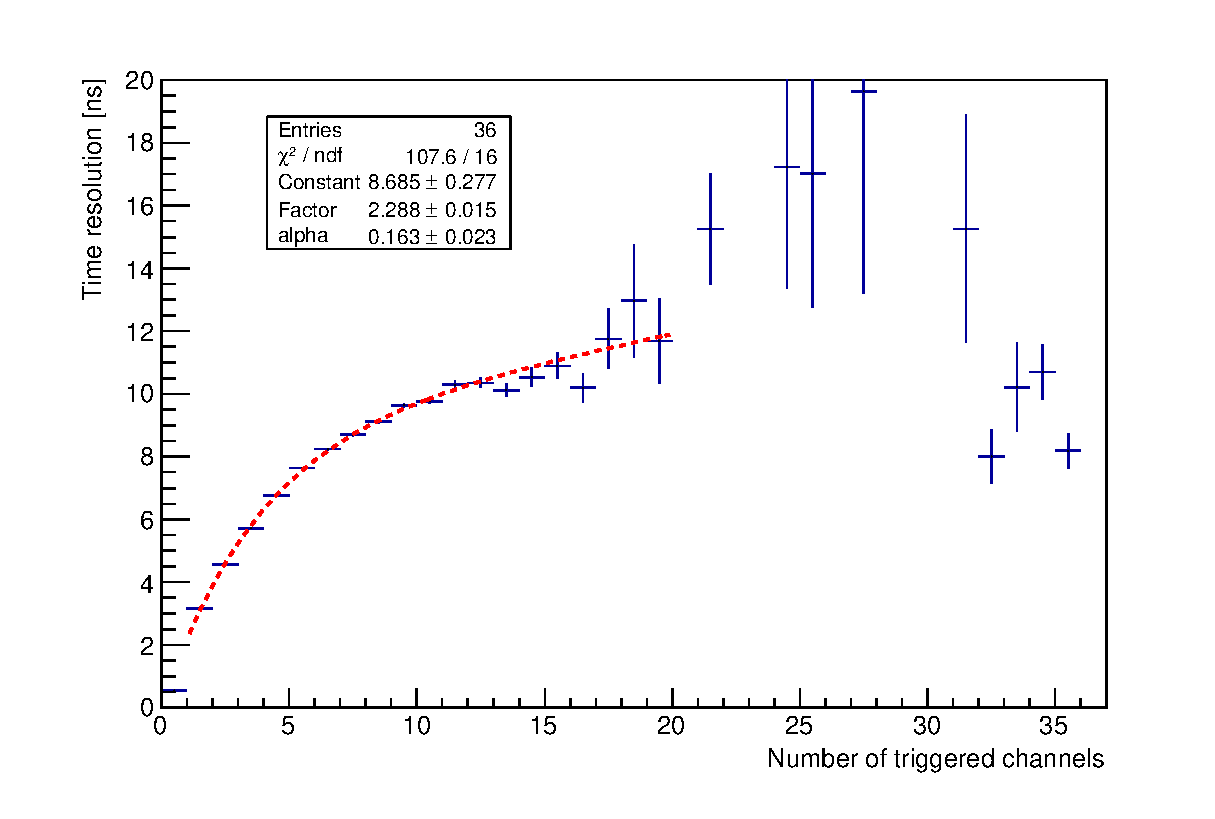
\includegraphics[width=0.5\textwidth]{fig/ParametrizationHits.eps}}
	\caption[]{\textbf{a}: The gaussian width is increasing with the number of triggered channels in a chip due to the remaining of the pedestal shift effect. The mean of the distribution shift slightly with increasing number of triggers but is neglected. \textbf{b}: Extracted width for each bins of number of triggered channels in a chip. The parameters are : A = 8.69 $\pm$ 0.28, $\epsilon$ = 2.29 $\pm$ 0.02 and $\alpha$ = 0.16 $\pm$ 0.02.}
	\label{fig:mc_para}
\end{figure}
The implemented parametrisation improve greatly the agreement between data and simulation for electrons as shown in figure \ref{fig:elec_sim_data_1}. A check has been done on the time of first hit distribution for muons and the effect improves also slightly the left tail of the distribution shown in figure \ref{fig:muon_ped_shift}.
\begin{figure}[htbp]
\begin{center}
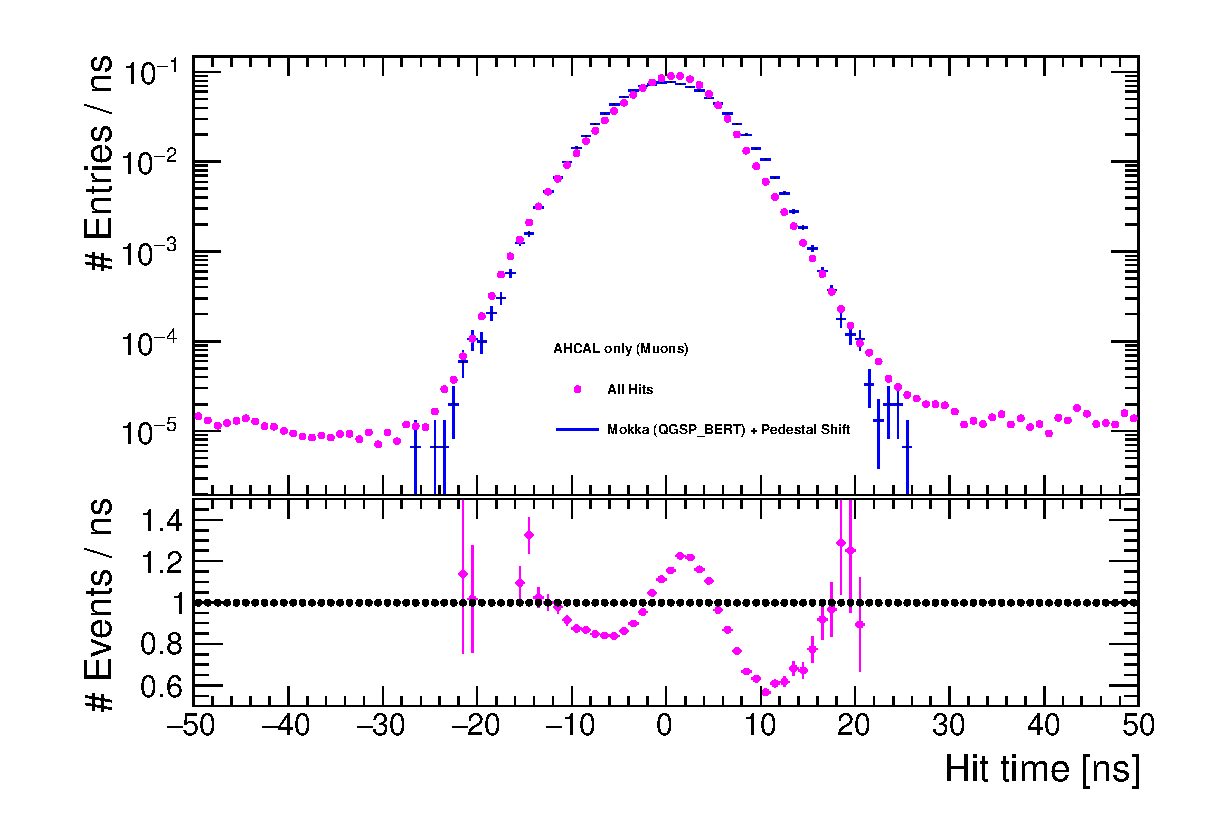
\includegraphics[width=0.6\textwidth]{fig/Comparison_SimData_Muons_PedShift.eps}
\caption{Time of first hit for data and simulation between -50 and 50 ns after the pedestal shift implementation. The left tail is in better agreement with simulation (up to 20\%) but degrades it for the right tail.}
\label{fig:muon_ped_shift}
\end{center}
\end{figure}
\newpage
\section{Study of noise on timing.}
\label{appendix:noise_timing}


\end{appendix}
\end{document}
